%%%%%%%%%%%%%%%%%%%% author.tex %%%%%%%%%%%%%%%%%%%%%%%%%%%%%%%%%%%
%
% sample root file for your "contribution" to a contributed volume
%
% Use this file as a template for your own input.
%
%%%%%%%%%%%%%%%% Springer %%%%%%%%%%%%%%%%%%%%%%%%%%%%%%%%%%


% RECOMMENDED %%%%%%%%%%%%%%%%%%%%%%%%%%%%%%%%%%%%%%%%%%%%%%%%%%%
\documentclass[graybox]{svmult}

% choose options for [] as required from the list
% in the Reference Guide

\usepackage{mathptmx}       % selects Times Roman as basic font
\usepackage{helvet}         % selects Helvetica as sans-serif font
\usepackage{courier}        % selects Courier as typewriter font
\usepackage{type1cm}        % activate if the above 3 fonts are
                            % not available on your system
%
\usepackage{makeidx}         % allows index generation
\usepackage{graphicx}        % standard LaTeX graphics tool
                             % when including figure files
\usepackage{multicol}        % used for the two-column index
\usepackage[bottom]{footmisc}% places footnotes at page bottom

% see the list of further useful packages
% in the Reference Guide

\makeindex             % used for the subject index
                       % please use the style svind.ist with
                       % your makeindex program

\hyphenation{sociotech-ni-cal}

%%%%%%%%%%%%%%%%%%%%%%%%%%%%%%%%%%%%%%%%%%%%%%%%%%%%%%%%%%%%%%%%%%%%%%%%%%%%%%%%%%%%%%%%%

\begin{document}

\title*{Embedding IoT in Large-scale Socio-technical Systems: A Community-Oriented Design in Future Smart Grids}
\titlerunning{Embedding IoT in Large-scale Socio-technical Systems} 

\author{Name of First Author and Name of Second Author}
% Use \authorrunning{Short Title} for an abbreviated version of
% your contribution title if the original one is too long
\institute{Name of First Author \at Name, Address of Institute, \email{name@email.address}
\and Name of Second Author \at Name, Address of Institute \email{name@email.address}}
%
% Use the package "url.sty" to avoid
% problems with special characters
% used in your e-mail or web address
%
\maketitle

\abstract*{In traditional engineering, technologies are viewed as the central piece of the engineering design, where the physical world consists of a large number of diverse technological artifacts. The real world, however, also comprises a huge amount of social components -- people, communities, institutions, regulations and everything that exists in the human mind -- that have shaped and been shaped by the technical components. Smart urban ecosystems are examples of such large-scale socio-technical systems that rely on technologies, particularly IoT, within a complex social context where the technologies are embedded. Despite that the two aspects are deeply intertwined, designing applications that embed IoT in large-scale socio-technical systems is slowly transitioning from a traditional engineering approach towards a socio-technical approach. The latter has not yet entered the mainstream of design practice. In this chapter, we present our experience of adopting a socio-technical approach in designing a community-oriented smart grid user application. The challenges, implications and lessons learned are discussed. The chapter is concluded by offering a set of good design principles derived from this experience, which are also relevant to the design of other smart urban ecosystems.}

%change the abstract above too
\abstract{In traditional engineering, technologies are viewed as the central piece of the engineering design, where the physical world consists of a large number of diverse technological artifacts. The real world, however, also comprises a huge amount of social components -- people, communities, institutions, regulations and everything that exists in the human mind -- that have shaped and been shaped by the technical components. Smart urban ecosystems are examples of such large-scale socio-technical systems that rely on technologies, particularly  Internet-of-Things (IoT), within a complex social context where the technologies are embedded. Despite that the two aspects are deeply intertwined, designing applications that embed IoT in large-scale socio-technical systems is slowly transitioning from a traditional engineering approach towards a socio-technical approach. The latter has not yet entered the mainstream of design practice. In this chapter, we present our experience of adopting a socio-technical approach in designing a community-oriented smart grid user application. The challenges, implications and lessons learned are discussed. The chapter is concluded by offering a set of good design principles derived from this experience, which are also relevant to the design of other smart urban ecosystems.}

\section{Introduction}
\label{sec:intro}

The traditional science and engineering philosophy is dominated by technological determinism, the idea that technology determines societal development \cite{Mody2006,Sawyer2014,Smith1994}. Within this reductionist view, technologies are the central piece of the engineering design, where the physical world consists of a large number of diverse technological artefacts. 
The plausibility of this view is challenged by the socio-technical systems view \cite{VanDam2012} which argues that technological and social development form a ``seamless web'' where there is no room for technological determinism or the autonomy of technological systems \cite{Fleischhacker2004}. 
%
The latter view is premised on the interdependent and deeply linked relationships among the features of technological artefacts or systems and social systems (i.e. the mutual constitution) \cite{Sawyer2014}, since the man-made world also comprises a huge amount of social components -- people, communities, institutions, regulations, policies and everything that exists in the human mind -- that have shaped and been shaped by the technological components \cite{Harari2014,VanDam2012}. 
In this view, engineering design is identified as a process through which technologies materialize into products, a process that substantively  shapes  and  reshapes  our  lives  and   societies and vice versa \cite{Kroes2008}. This focus on socio-technical interconnectedness becomes even  more  visible in designing new emerging technologies \cite{Kroes2008}.  

%With the world's rapid growing population\footnote{In 2014, 54\% of the world's population resides in urban areas. This figure was 30\% in 1950, and is project to be 66\% by 2050 \cite{UN2014}.}
Smart cities, for example, use technologies such as Internet-of-Things (IoT) within a large complex social context where they are embedded. The goal is to facilitate the coordination of fragmented urban sub-systems and to improve urban  life experience \cite{Glasmeier2015}. 
% 
<<<<<<< HEAD
The rise of the IoT has important socio-technical implications for people, organizations and society -- it is obvious that connecting devices is possible, we yet know little about its implications \cite{Shin2014}. A socio-technical perspective can be insightful when looking at dynamic technological development and when considering sustainable development \cite{Shin2014}. Although socio-technical systems have been studied for decades, socio-technical approaches are relatively new to the design and systems engineering communities \cite{Baxter2011,Norman2015,Sawyer2014}. Such approaches are not widely practised despite growing interests \cite{Baxter2011}. %and slow transition
=======
The rise of IoT has important socio-technical implications for people, organizations and society. It is obvious that connecting devices is technically possible, we yet know little about its implications \cite{Shin2014}. A socio-technical perspective can be insightful when looking at dynamic technological development and when considering sustainable development \cite{Shin2014}. Although socio-technical systems have been studied for decades, socio-technical approaches are relative new to the design and systems engineering communities \cite{Baxter2011,Norman2015,Sawyer2014}. Such approaches are not widely practised despite growing interests \cite{Baxter2011}. %and slow transition
>>>>>>> civis

\begin{svgraybox}
Through this chapter, we review the literature and present our experience of adopting a socio-technical approach in designing a community-oriented smart grid user application. We discuss the challenges, implications and lessons learned from this design experience, and conclude the chapter by offering a set of good design principles which are also relevant to the design of other smart urban ecosystems. 

%The transition of energy system -to- smart energy system, passive user to active / engaged user
\end{svgraybox}


\section{Designing in Large-scale Socio-technical Systems}
\label{sec:design}
% Always give a unique label
% and use \ref{<label>} for cross-references
% and \cite{<label>} for bibliographic references
% use \sectionmark{}
% to alter or adjust the section heading in the running head

The term ``socio-technical'' embodies both a research perspective and a subject matter \cite{Lee2001}.
The socio-technical systems view can be articulated as the recognition of three fundamental concepts \cite{Sawyer2014} as follows. 
%
First, the \textit{mutual constitution of people and technologies}. This mutual constitution generates complex and dynamic interactions among technological capacities, social norms, histories, situated context, human choices and actions, etc. 
%
Second, the \textit{contextual embeddedness of the mutuality}, where the context is not taken as fixed or delineable. There are dynamic situational and temporal conditions that influence 
mutual adaptations throughout the course of design, development, deployment and uses of the system of interest. 
% 
Third, the \textit{importance of collective action}, the joint pursuit of one or more shared (potentially conflicting) goals by two or more interested parties such as problem owners, shareholders, users, communities affected (without implying positive or negative outcomes). The collective action shapes and is shaped by both the context and the technological components. 

Researchers who hold a socio-technical systems view investigate more than just the technological system or just the social system or even the two side by side, but also the phenomena that emerge when the two interact \cite{Lee2001}. A socio-technical approach tries to abstain from oversimplifications that seek a single or dominant cause of change, but studies the complexity, dynamic and uncertainty in the networks of institution, people and technological artifacts in the process of technologically involved change \cite{Sawyer2014}. 
%
Taking a socio-technical approach towards design has a number of implications for (i) the formulation of the design problem, (ii) the products of the design process, and (iii) the design process itself (BootCamp, BC?).

\begin{svgraybox}

Then the section proceeds with discussing the three implications (1) making relation to the three fundamental concepts (2) using the literature mentioned (can be expanded) in the next grey box 

\runinhead{Understanding and formulation of the design problem or situation}

The understanding and formulation of the design problem 

 It is not straightforward what needs to be taken into consideration in relation to the design. What systems boundaries to choose. the question of systems boundaries is an issue for technical systems and even becomes more difficult for social technical systems
what are the issues to be addressed.[BC]

Ill-structured problem

\runinhead{Products of the design process} these not only consists of technological artifacts but also may include rules for behaviour, policies, etc. through which the designer wish to intervene in social-technical systems. what is it that we are designing? 

\runinhead{Design process} The design process can be seen as a decision-making process where the problem owners, shareholders, users, etc. participate to represent their interests. It is often conceived and implemented in participatory decision-making processes actively involving stakeholders

Large-scale socio-technical systems are often not designed as a whole but incrementally ``piece by piece'' evolving from legacy systems (BC). Designers are therefore working \textit{in} the context of some socio-technical system with the intention of changing or improving some part of that system [BC]. This means that what matters more in the design is the design process itself, more than the ``final status'' of the system \cite{Shin2014, need more ref} because the socio-technical system keeps evolving and exhibits emergent behaviour \cite{Nikolic2009}. An important  goal of the design process is to make the design (a product or system) relevant to the evolving context \cite{Shin2014, need more ref} as social and technical artifacts exist within their socio-technical context [BC]. 

\end{svgraybox}



\begin{svgraybox}
can be put in the discussion: 
acontextual and detemporalized perspective approaches , general solution ., is self-limiting 
focus on situating work and seek to examine all contextual factors , this types of inquiry attempt to construct a holistic view of context: one that does not diminish or remove contextual elements, even those with limited influence. 
paying little attention to the environment of the organization and temporal dimension of technological innovation  \cite{Sawyer2014}
\end{svgraybox}


\begin{svgraybox}
Use and combine content in: (the literature can be connected, e.g. problems mentioned in Norman and Baxter  can be mapped to the four layers in Whitworth )
\begin{enumerate}
\item \cite{Norman2015} (design problems in large-scale socio-technical systems) and 
\item \cite{Baxter2011} (socio-technical approach to systems engineering)
\item \cite{Whitworth2009} (four system levels of Socio-tehnical systems); 
\item \cite{Shin2014} (a very good article about IoT, socio-technical perspective )
\item see also https://medium.com/rettigs-notes/notes-on-sociotechnical-systems-design-178f161bc9e8 
\end{enumerate}
\end{svgraybox}



\section{IoT as a Socio-technical System}
\label{sec:IoT_socio-techical}

\begin{svgraybox}
	Through this chapter, we review the literature on
	
	1 IoT as socio-technical system and
	
	2 how IoT can support the design and development of the smart grid.
\end{svgraybox}

Since 1999, when Ashton \cite{ashton2011internet} coined the term \textbf{Internet of Things (IoT)}, while he was introducing RFID technology in the context of supply-chain management, the meaning of the term has evolved. Today, International Telecommunication Union (lTU) defines IoT as the worldwide network of interconnected objects uniquely addressable based on standard communication protocols. Such a definition focuses only on the technical side of IoT. From the technical aspect, the IoT can be divided into three following layers:
\begin{itemize}
	\item comprehensive sensing (perception layer),
	\item reliable transmission (network layer), and
	\item intelligent processing (application layer).
\end{itemize}
Nevertheless, the envisioned IoT represents a socio-technical, instead of an only technical system, as the interconnected objects are intended to interact also with people and society \cite{atzori2014smart,Shin2014}. 
However, the focus among engineers and computer scientists when discussing IoT was mainly on the technical side, as is the case with other socio-technical systems.
Interestingly, even some of the ideas for the \textit{Social IoT (SIoT)} \cite{atzori2012social,guinard2010sharing,atzori2014smart} discuss the convergence of social networks with IoT mainly with the intention to optimize the interactions among the IoT objects. There is often very little attention placed in such studies on the interrelationship of IoT with the human psychological and social aspects \cite{atzori2012social,guinard2010sharing}. 

The discussion on IoT should also cover another term that is often used interchangeably -- \textbf{ubiquitous computing}, coined by Weiser \cite{weiser1991computer}. Ubiquitous computing is defined as ``the physical world that is richly and invisibly interwoven with sensors, actuators, displays, and computational elements, embedded seamlessly in the everyday objects of our lives, and connected through a continuous network'' (ibid.). In other words, while the Internet has led to the interconnection of people at an unprecedented scale, the IoT is expected to interconnect also the objects around us, leading to a smart environment \cite{gubbi2013internet}. %We see that researches talking about IoT mainly describe connected devices, while ubiquitous computing focuses on the smart environment in which computing is pervasive. 
%Hence, the two terms take a different stance and focus on different aspects of what is envisioned to become the \textit{Future Internet}. 
The IoT vision put forward by Weiser \cite{weiser1991computer} led to a fruitful new field within computer science (ubiquitous computing). In particular, the original vision suggested that ubiquitous computing can lead to an environment that is predicting and adapting to the people's needs, while the people were considered passive elements (i.e., technological determinism). However, Rogers \cite{rogers2006moving} offered a constructive critique of this vision. Namely, Rogers argued that we should move from a \textit{computing approach} (technical aspects) to a \textit{human approach} (social aspects) in developing the smart environment. Rogers argues: ``To make this happen, however, requires moving from a mindset that wants to make the environment smart and proactive to one that enables people, themselves, to be smarter and proactive in their everyday and working practices.''

The effects of the critique, such as the one by Rogers, are seen in researches increasingly adopting the design of IoT as a socio-technical artifact \cite{ning2011future,guo2012opportunistic,Shin2014,tomasini2017effect}. One human-centric vision is illustrated by the \textit{Opportunistic IoT} \cite{guo2012opportunistic,guo2013opportunistic}. The authors explain that in addition to object-object interaction, the IoT design should consider human-object, human-environment and human-human interactions. Moreover, it is also recognized that the IoT design needs to consider different aspects of human behaviour, such as mobility \cite{tomasini2017effect}, preferences \cite{kowshalya2016community}, and homophily \cite{atzori2012social}. In the light of such ideas, Ortiz et al.\ \cite{ortiz2014cluster} revisit previously introduced ideas of {SIoT} (that still treat IoT only as technical system) and provide a more complete vision of it -- one that treats the IoT as a socio-technical system.

\begin{comment}
	\sidecaption
	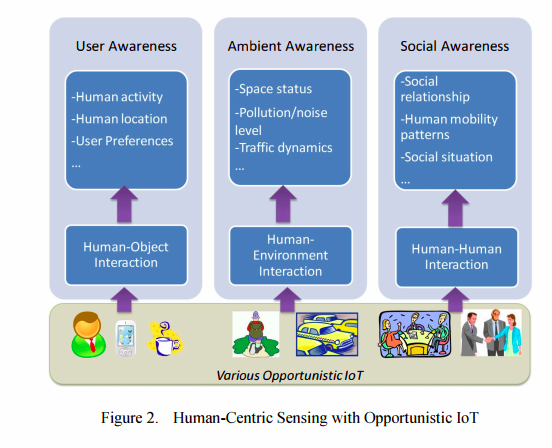
\includegraphics[scale=.55]{img/opprtunisticIoT}
	\caption{Human-centric Opportunistic IoT \cite{guo2012opportunistic}}
	\label{fig:opportunisticIoT} 
\end{comment}

Some of the key ideas in which the visions of IoT as a socio-technical system (SIoT) expand on those visions that treat it only as a technical system are the following. SIoT visions argue that the efforts should be placed on using and integrating the IoT in society and on the user-level, and building new communities of users and technology while considering actual adoption possibilities (versus designing intrusive technology that will not be used in the end). Moreover, the emphasis is on contextual design, so that IoT will be adapted to different psychological, social, legal, policy and other types of factors. Finally, people have to be empowered to embrace the IoT technologies with awareness raising, proper policies and  human-centered design \cite{ning2011future,Shin2014}.


\subsection{IoT for the Smart Grid}
\label{sec:IoTSG}
One of the key application areas of IoT is envisioned for the \textbf{smart grid}. In China, in particular, the largest portion of the IoT market is planned for the development of the smart grid \cite{shin2014socio}. Yun and Yuxin \cite{yun2010research} discuss the possibilities of the IoT to bring about the {smart grid} through sensors, novel telecommunications and computing technologies. The sensors, such as smart, temperature, and illumination meters can collect energy and environmental data. They can also form a high-speed, real-time and bidirectional connection between the consumers, utilities and the electrical grid. Such an improved data collection and communication can support the decision making and in turn improve the overall efficiency of the grid. Interestingly, the technology at the heart of the IoT, the Internet itself, consumes up to 5\% of the total energy spent today in the world. Given the expectation of connecting billions of new devices, this consumption is expected to raise \cite{gubbi2013internet}.	Hence, in addition to its role in optimizing the energy grid, the IoT design itself needs to place accent on sustainability.

%Different innovation layers can be used to describe the smart innovation and development characteristics within the smart cities \cite{zygiaris2013smart}. IoT should play an important role in several of those layers: from the interconnection layer with a number of sensors and actuators, through the integration layer monitoring those smart devices, to the intelligent applications layer making use of the real-time data. 

 IoT can support both the dimensions of demand and supply of energy in the smart grid. Tackling the demand should involve the users \cite{verbong2013smart}. While the focus on technology is still too strong and some smart grid players still perceive the users themselves as the barriers to the smart grid development process, they instead need to understand to what extent the users can act as a solution to the sustainability pathway. IoT is an integral technology in the \textit{smart residential buildings} \cite{schatten2014smart,zygiaris2013smart}. The smart devices that are interconnected and installed in smart buildings, such as smart energy, temperature, and illumination meters are enablers of the smart homes.

IoT is predicted to enable transparent energy consumption information of different services in \textit{smart cities}: from lighting, through public transport, to heating and air conditioning of public spaces \cite{zanella2014internet}. Moreover, the real-time, bidirectional connectivity between the utilities, grid and the users is suggested to lead to the improved overall efficiency of the grid \cite{yun2010research,li2011applications}. Similarly as with IoT in general, we also find visions of smart grid that employ social networks on top of interconnected devices, in this case, the smart meters \cite{ciuciu2012social}. Devices, in general, in the future smart homes and cities are expected to cooperate, actively share their energy and participate in building wide energy management systems \cite{karnouskos2010cooperative}. 

It is apparent how in such a context, where IoT meets the smart grid, innovative services and business applications emerge, but also security, privacy and trust gain novel importance.




\section{CIVIS: A Community-Oriented Design in Future Smart Grids}
\label{sec:civis}

Since more than two decades the ongoing and long-term energy transition shifted the energy domain
towards decentralization, distributed production and renewable sources \cite{rifkin_third_2011,sovacool_how_2016}. Several general and intertwined aspects contribute to this transition: 
(\textit{i}) the awareness of the inherent complexities that exist among energy systems, societies 
and the environment \cite{bulkeley_bringing_2012,umbach_global_2010}; (\textit{ii}) the
widespread diffusion of new, enhanced technologies and their hybridization with contemporary ICTs 
\cite{putrus_smart_2013,schick_innovating_2013}; (\textit{iii}) the pursuit of national and 
supranational energy policies around energy efficiency, sustainability and low carbon emissions 
\cite{da_graca_carvalho_eu_2012}; and (\textit{iv}) the emergence of new actors in the energy value 
chain, such as energy cooperatives and energy communities \cite{viardot_role_2013}, or the 
transformation of old ones, such as housing associations, and amateur energy managers 
\cite{hasselqvist_linking_2016}.

CIVIS work took place under European Union’s interest to support energy transition by tackling the 
so called societal challenge of efficient energy. The vision of smart grids and the use of ICTs were 
the main drivers for the project's ambition to reconfigure the relationships among traditional and 
emerging actors in the energy value chain -- \textit{i.e.} distributors, producers, retailers and 
prosumers, cooperatives. In particular, CIVIS was a three year, EU 
project\footnote{\url{http://cordis.europa.eu/project/rcn/110429\_en.html}} funded under the 
\textit{FP7 Smart Cities} framework, that pursued the design, prototyping and real-life testing of 
a platform for the improvement of energy behaviours in the domestic sector. The project was 
structured around three main areas of interest -- \textit{i.e.} energy, ICT, and social innovation 
-- and organized into three broad phases that roughly overlapped with the project years and that 
ensured a close interaction with the local realities and contexts of the pilots: (\textit{i}) an 
exploratory phase, used to align CIVIS’ overarching objectives with the local contexts’ needs;
(\textit{ii}) a prototyping one, which concerned the actual design and development of the platform 
(from data monitoring devices to the front-end applications); and (\textit{iii}) a final testing 
phase which included the full scale deployment of the platform in the pilots for usage and 
assessment purposes.
Therefore, in CIVIS the possibilities for a socio-technical approach were present by design
in the formal structure and description of the project.
Furthermore, the composition of the consortium included the diversity of disciplinary backgrounds
and profiles -- \textit{i.e.} engineers, computer scientists, designers, and sociologists --
that was necessary for tackling the evolving shaping and
understanding of the socio-technical system from multiple perspectives (See Fig. \ref{fig:sts_levels}).

Below we clarify how CIVIS adopted %is the right word?? (used?)
a socio-technical approach in practice. We provide an overview of the context of the design situation,
we summarize the collaborative design process that was put in place, and we present
the main outcomes, which allow to appreciate CIVIS socio-technical system both in
its technical and social levels.  

\subsection{Understanding and Formulation of the Design Situation}

Concretely, CIVIS' platform goals were to increase energy awareness, by making energy behaviours more visible, to promote
environmental and social values, to increase citizens' know-how about sustainable consumption, and to help
them in improving energy behaviours in their everyday life and together with local communities.

These interests built upon existing research and emerging trends.
For instance, research topics linking the potential of Social Networks (SNs) with that of smart grid applications 
have caught great attention in recent years, following the success of several popular platforms 
\cite{Boslet2010,Chima2011,Erickson2012,Fang2013,Huang2015}. 
Some conducted surveys to understand user needs for energy services combining SNs \cite{Silva2012}. 
Some studied connecting smart meters (or smart homes) for energy management and
sharing \cite{Ciuciu2012,Steinheimer2012}. 
Simulation models are developed to study value-added web services \cite{De-Haan2011,Lei2012,Chatzidimitriou2013} and to 
demonstrate the feasibility of coordination in meeting energy targets \cite{Worm2013,Skopik2014}.
Finally, works that visualize smart meter and appliance-level consumption data to enable comparative 
feedback among households are also increasing \cite{Petkov2011,Weiss2012,Dillahunt2014}.

However, we also wanted the overarching purpose, the underlying infrastructure and the core features of 
CIVIS Platform to be able to integrate 
into rather different contexts, to meet diverse needs and expectations as well as to serve various 
types of user. This is why, in CIVIS, the pilot sites were understood more as sources of collaborative design and development,
rather than just as passive recipients of a technology to be tested.  

Italy and Sweden hosted two pilots each. In the former, the work focused on cooperative owned 
electricity provision. In the latter, it concerned housing cooperative's energy management in 
apartment buildings and townhouses.  
In brief, the two municipalities of Storo and San Lorenzo, in Trentino Alto-Adige (a region in 
north-west Italy), included the Italian pilots. Here, two electric cooperatives, producing and 
selling 100\% renewable energy to their associate members, together with two samples of recruited 
associate member households acted as the main stakeholders. The regional distribution system 
operator (DSO), the institutional representatives of the two municipalities and two local cultural 
associations participated as stakeholders in various phases of the project, by providing knowledge 
and support for technical aspects related to energy and households engagement.
Similarly, the area of Stockholm hosted the two Swedish pilots. One involved the residential and 
central neighbourhood of Hammarby Sj\"{o}stad, which included apartment buildings owned by housing 
cooperatives\footnote{In Sweden, those who buy an apartment must join a corresponding \textit{housing cooperative} that owns and maintains the estates. The 
members of a cooperative annually elect a board that makes energy related decisions on behalf of 
the members.}. Recruited households from the cooperatives and cooperatives' board members acted
as key stakeholders here. % Was YouPower released in Fardala at all? Do we want to explicitly talk about Fardala?
The other pilot concerned a townhouse area in the outskirts of Stockholm: F\aa{}rdala. In this townhouse area the 
local residents’ association and some of its member households participated to CIVIS.

Ultimately, and at the general level, the design problem areas converged on two different sets of problems
depending on the two countries. In Italy, the platform had to integrate into energy communities to support
efforts of demand-side management\footnote{\textit{E.g.} Moving peaks of electricity demand, towards peaks of local energy
production or, in other words, improving the self-consumption capabilities of the electric cooperatives and
their associate members}. In Sweden, it had to support knowledge sharing about energy management practices at building
and apartment levels.

TODO

\paragraph{Evaluation} After a successful deployment, YouPower was evaluated in the test sites in Sweden and Italy. We collected in parallel, the data on user engagement with the app and on energy prosumption. The initial evaluation revealed how the Trentino residents engaged with a weather feature that predicts the solar energy production levels, while the Stockholm housing association managers used the community features to engage with the residents and connect with other managers. 

Some of the tangible results in the Italian test site include the savings in the electricity and heating energy spent or produced \cite{civics}:
\begin{itemize}
	\setlength{\itemsep}{0mm}
	\item percent	of	self-consumption	of	 the	PV	self-produced energy	 is	 increased	 for more than	50\% of the	users	comparing	to	the period before CIVIS;
	\item electricity	consumption	from the	grid	is	reduced for the same period for	more than	50\% of the	consumers;	
	\item 	total	 electricity	 consumption	 (including both, from	the grid	 and	the PV	 self-consumption)		is	reduced for the same period for	more than	50\% of the	consumers;	
	\item  the users spent less than 11\% of hours in overheating their spaces.\footnote{The	heating behaviour	 of	 CIVIS	 users (control	 of	 space	 heating),	 met	 the	recommended	standard	values.}
\end{itemize}

The housing cooperatives (BRF; bostadsr\"attsf\"orening	in	Swedish) in Stockholm conducted following actions as a result of the YouPower use \cite{civics}:

\begin{itemize}
	\setlength{\itemsep}{0mm}
	\item BRF	Grynnan: adjustments of	ventilation	system and	turning	off	the	outdoor	ice	melting	system (resulting in	reductions	in	heating);
	\item BRF	 Sj\"ostaden	 1: extra	 insulation	 added	 to	 the	 roofs in	May	2015	(lead	to	a	decrease	in	heating	consumption);	 installation	 of	 heat	 recovery	 heat	 pumps	 in	 February	 2016 (lead	 to	 some	 increase	 in	 electricity	 consumption	 but	 the	 overall	savings);
	\item BRF	\"Alven: ventilation	optimization due to lower thermal comfort,	however	the	energy	use	went	up;
	\item BRF	 Seglatsen: installation of recovery	heat	pumps	in	 the	building (reduction in	 the	heating	consumption	by	around	60\%, and since electrcitiy consumption increased, overall savings are	about	40\%).	
	\item BRF	 Hammarby	 Kanal:	 ventilation optimization;
	\item BRF	 Hammarby	 Ekbacke: a goal	 based	 energy	 reduction in	a	new	business	model	for	the	housing	associations	where	 they do not	 have	 to	 pay upfront	costs	for	the energy 	actions, and then part	of	the	savings	goes to	the	 ESCO (European Skills, Competences, Qualifications and Occupations)	 for	 a	 fixed	 time	 period.	
\end{itemize}


To assess the long term effectiveness of the CIVIS social energy intervention,  after a certain period of time, it would be beneficial to fuse the collected data from the app with those about the consumption/prosumption. 

\paragraph{Limitations} The initial lack of data due to acquisition and privacy issues in the residential setting was among the main limitation in this project. We installed the IoT sensors to collect additionally needed data for using the introduced app. 

\subsection{Design Process (or participatory design?)}

% \begin{svgraybox}
% [note by GP] Giacomo can write most of this part. 
% \end{svgraybox}

CIVIS design process was theory-driven, user-centered, collaborative and iterative. Indeed, a
literature review was carried early in the project on the intervention strategies and the social smart
grid applications for the promotion of environmental behavior change. This provided an initial, broad set
of possibilities which had been iteratively, assessed, refined and improved throughout the design process with
the collaboration and participation of basically all actors affected by it.

The rationale behind this approach rested on the conviction that applying a user-centered and
collaborative design process to the development of large socio-technical system has positive
theoretical, practical and ethical implications \cite{Greenbaum1993,Boedker2004} by, for instance, increasing users engagement,
usability and integration into existing local conditions \cite{Brynjarsdottir2012,Dick2012,Pierce2012}.

Along the three years, the process unfolded as a complex and articulated network of meetings and artefacts
which strived to align the interests of different stakeholders involved, from porject partners to
local stakeholders and end-users. We organized brainstorming sessions and design workshops, we run
exploratory and evaluation focus groups with end-users in the test sites, as well as design workshops.
Due to the limited space, here we only streamline the main aspects of the process and direct readers to
\cite{poderi_disentangling_2017} for a detailed study on how the process shaped the main
outcomes of CIVIS. % Do we want to refer to CIVIS as the project, or CIVIS platform or avoid alltogether to refer to it as an entity (once we have introduced it)

In short, a constant work of alignment took place at an high level of abstraction mainly thanks to
the use of user stories as key boundary object among stakeholders,
expertises and local contexts. At a more concrete level, a set of platform features was prototyped in simple mock-ups
and also used as a basis for discussion. These underwent iterative rapid prototyping which
produced wireframes as better visual guides that could be more effectively communicated to end-users.
Prior and after each iteration, exploratory activities on how to proceed and evaulation sessions for their outcomes
took place in different venues and with different stakeholders -- \textit{e.g.} from participants in
an environmental event \cite{Barssi2015} to stakeholders at test sites, and by groups of experts.


\subsubsection{User stories}

We adopted the tool of user stories \cite{Kankainen2012} from Software Engineering and adapted it to the context of our
socio technical system. User stories crossed CIVIS both horizontally (to the
scope of the work packages) and vertically (to the needs of the two countries). In short, each user
story identified a realistic scenario, a main scope of the energy intervention, the supporting ICT tools,
and the central social dynamics. During the three years we drafted, refined, merged, abandoned and
finalized them as part of our constant work of alignment and negotiation. We discussed them in internal
workshops, round-tables with stakeholders, and focus-groups with participant end-users; we circulated
them to software engineers and platform designers; we publicly presented them for feedback and used them
as frames for collaborative workshops. They represented evolving artefacts that we consolidated in formal
versions at the end of every year of activity. 


\subsubsection{Stakeholders meetings} % MAYBE TURN THESE INTO \PARAGRAPHS ?

%
\begin{figure}
      \begin{center}
        \begin{minipage}[htb]{0.43\linewidth}    
        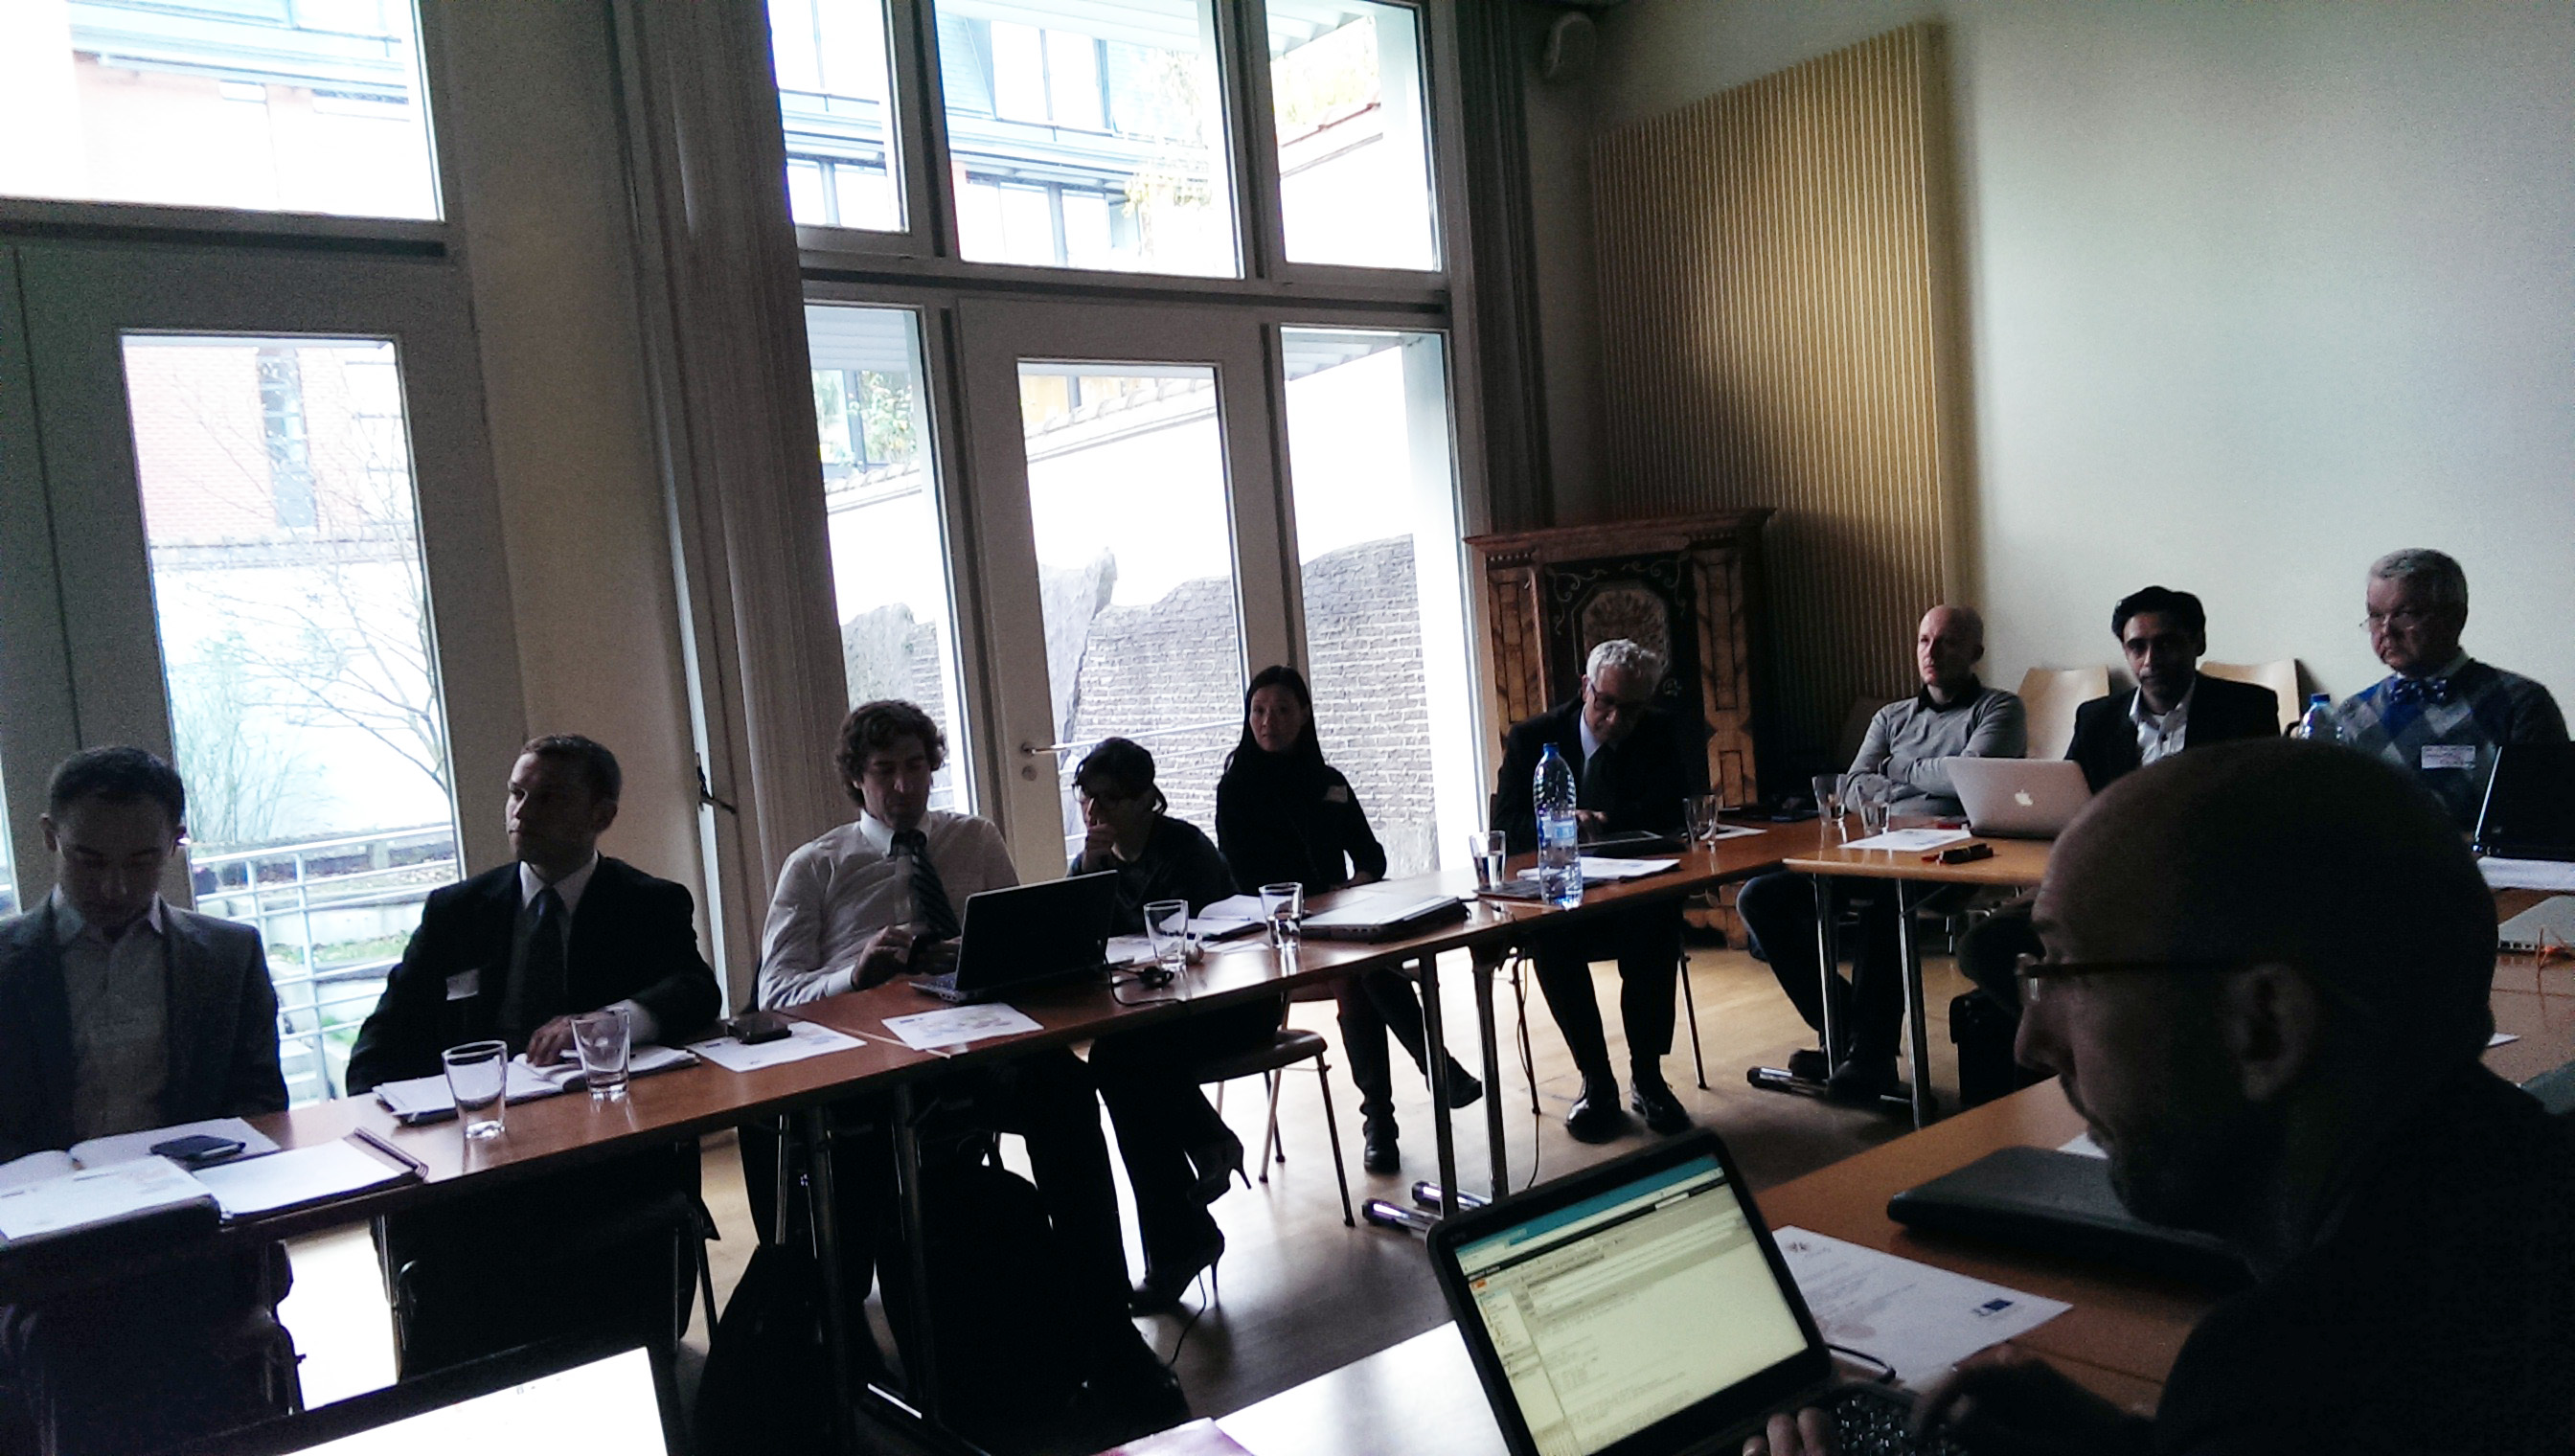
\includegraphics[width=1\linewidth]{img/Stkh_plenary1.jpg}
        \end{minipage}
 	\hfill 
         \begin{minipage}[htb]{0.55\linewidth}    
	        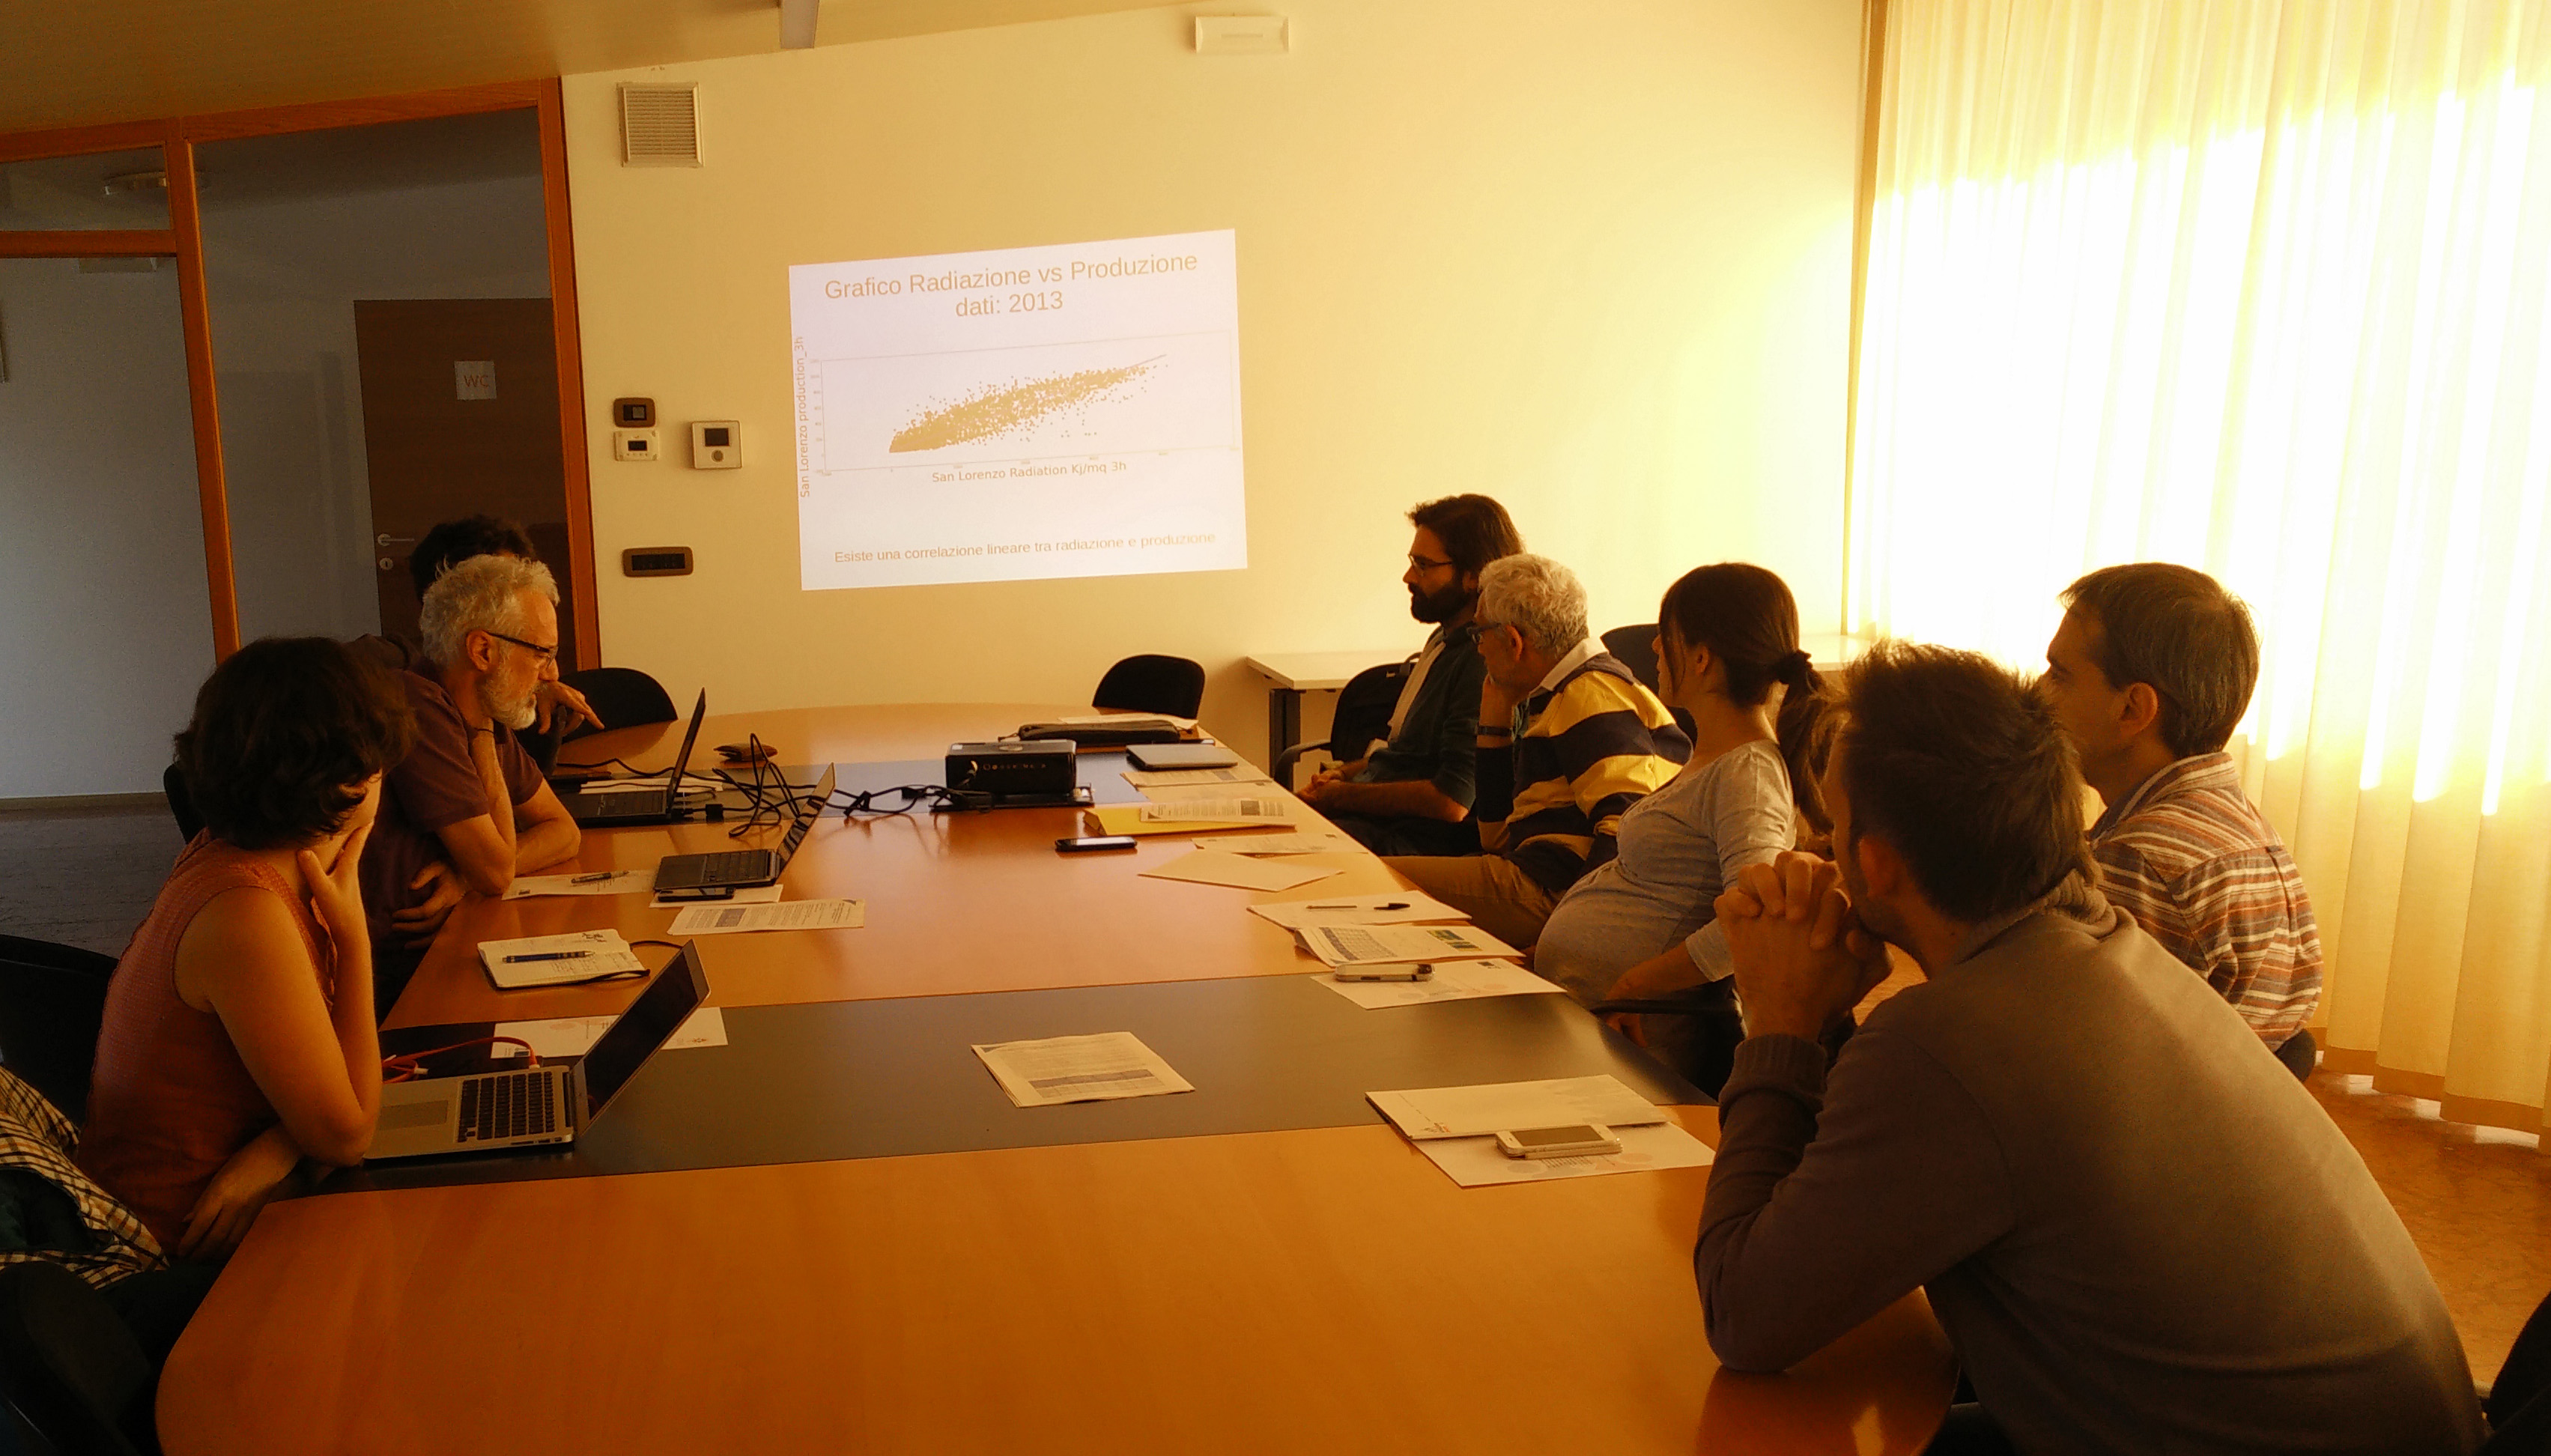
\includegraphics[width=1\linewidth]{img/Stkh_meeting_tou_crop.jpg} 
                \end{minipage}
      \end{center}
    \caption{(a) A moment during one of the first project plenary meetings, where local stakeholders from the pilot sites took part; (b) Stakeholder meeting between some of the technical project partners and
    local stakeholders in Italy, to discuss the aspects of demand-side management.
}
\label{fig:stkh_meetings}
\end{figure}
%

These were held primarily at the level of the pilot sites, by involving CIVIS technical figures and the
key local energy stakeholders. Roughly, they were held quarterly, although at the project's onset and during
the most intense `design phase' of the work, they occurred more frequently.

These meetings proved helpful for agreeing on the project overarching objectives at the local levels, but also
for understanding the feasibility and rationality of the choices for the social and technical aspects of the platform.
For instance, it required long discussions and negotiation the identification and selection of the energy monitoring devices to be installed in
participants households for enabling the proper granularity and availability of energy data. Indeed,
the suitability of these devices could not be assessed at a technical level only (\textit{e.g.} cost/efficiency, type of data,
reliability, protocols). Typology of end-users, acceptability, and housing conditions \footnote{ In italy, participants were older and less tech-savy, living in own
independent, large houses; while in Sweden they were relatively younger and more tech-savy, but living in smaller apartments in residential buildings.}
also played an important role. 

%
% Another example that can be brought up relate to the availability of DSO data, which took a long time to be clarified and it also influenced/related a lot with the
% possible/desired features of the platform.
%


\subsubsection{Focus groups} % MAYBE TURN THESE INTO \PARAGRAPHS ?

%
\begin{figure}[h!]
	\centering
	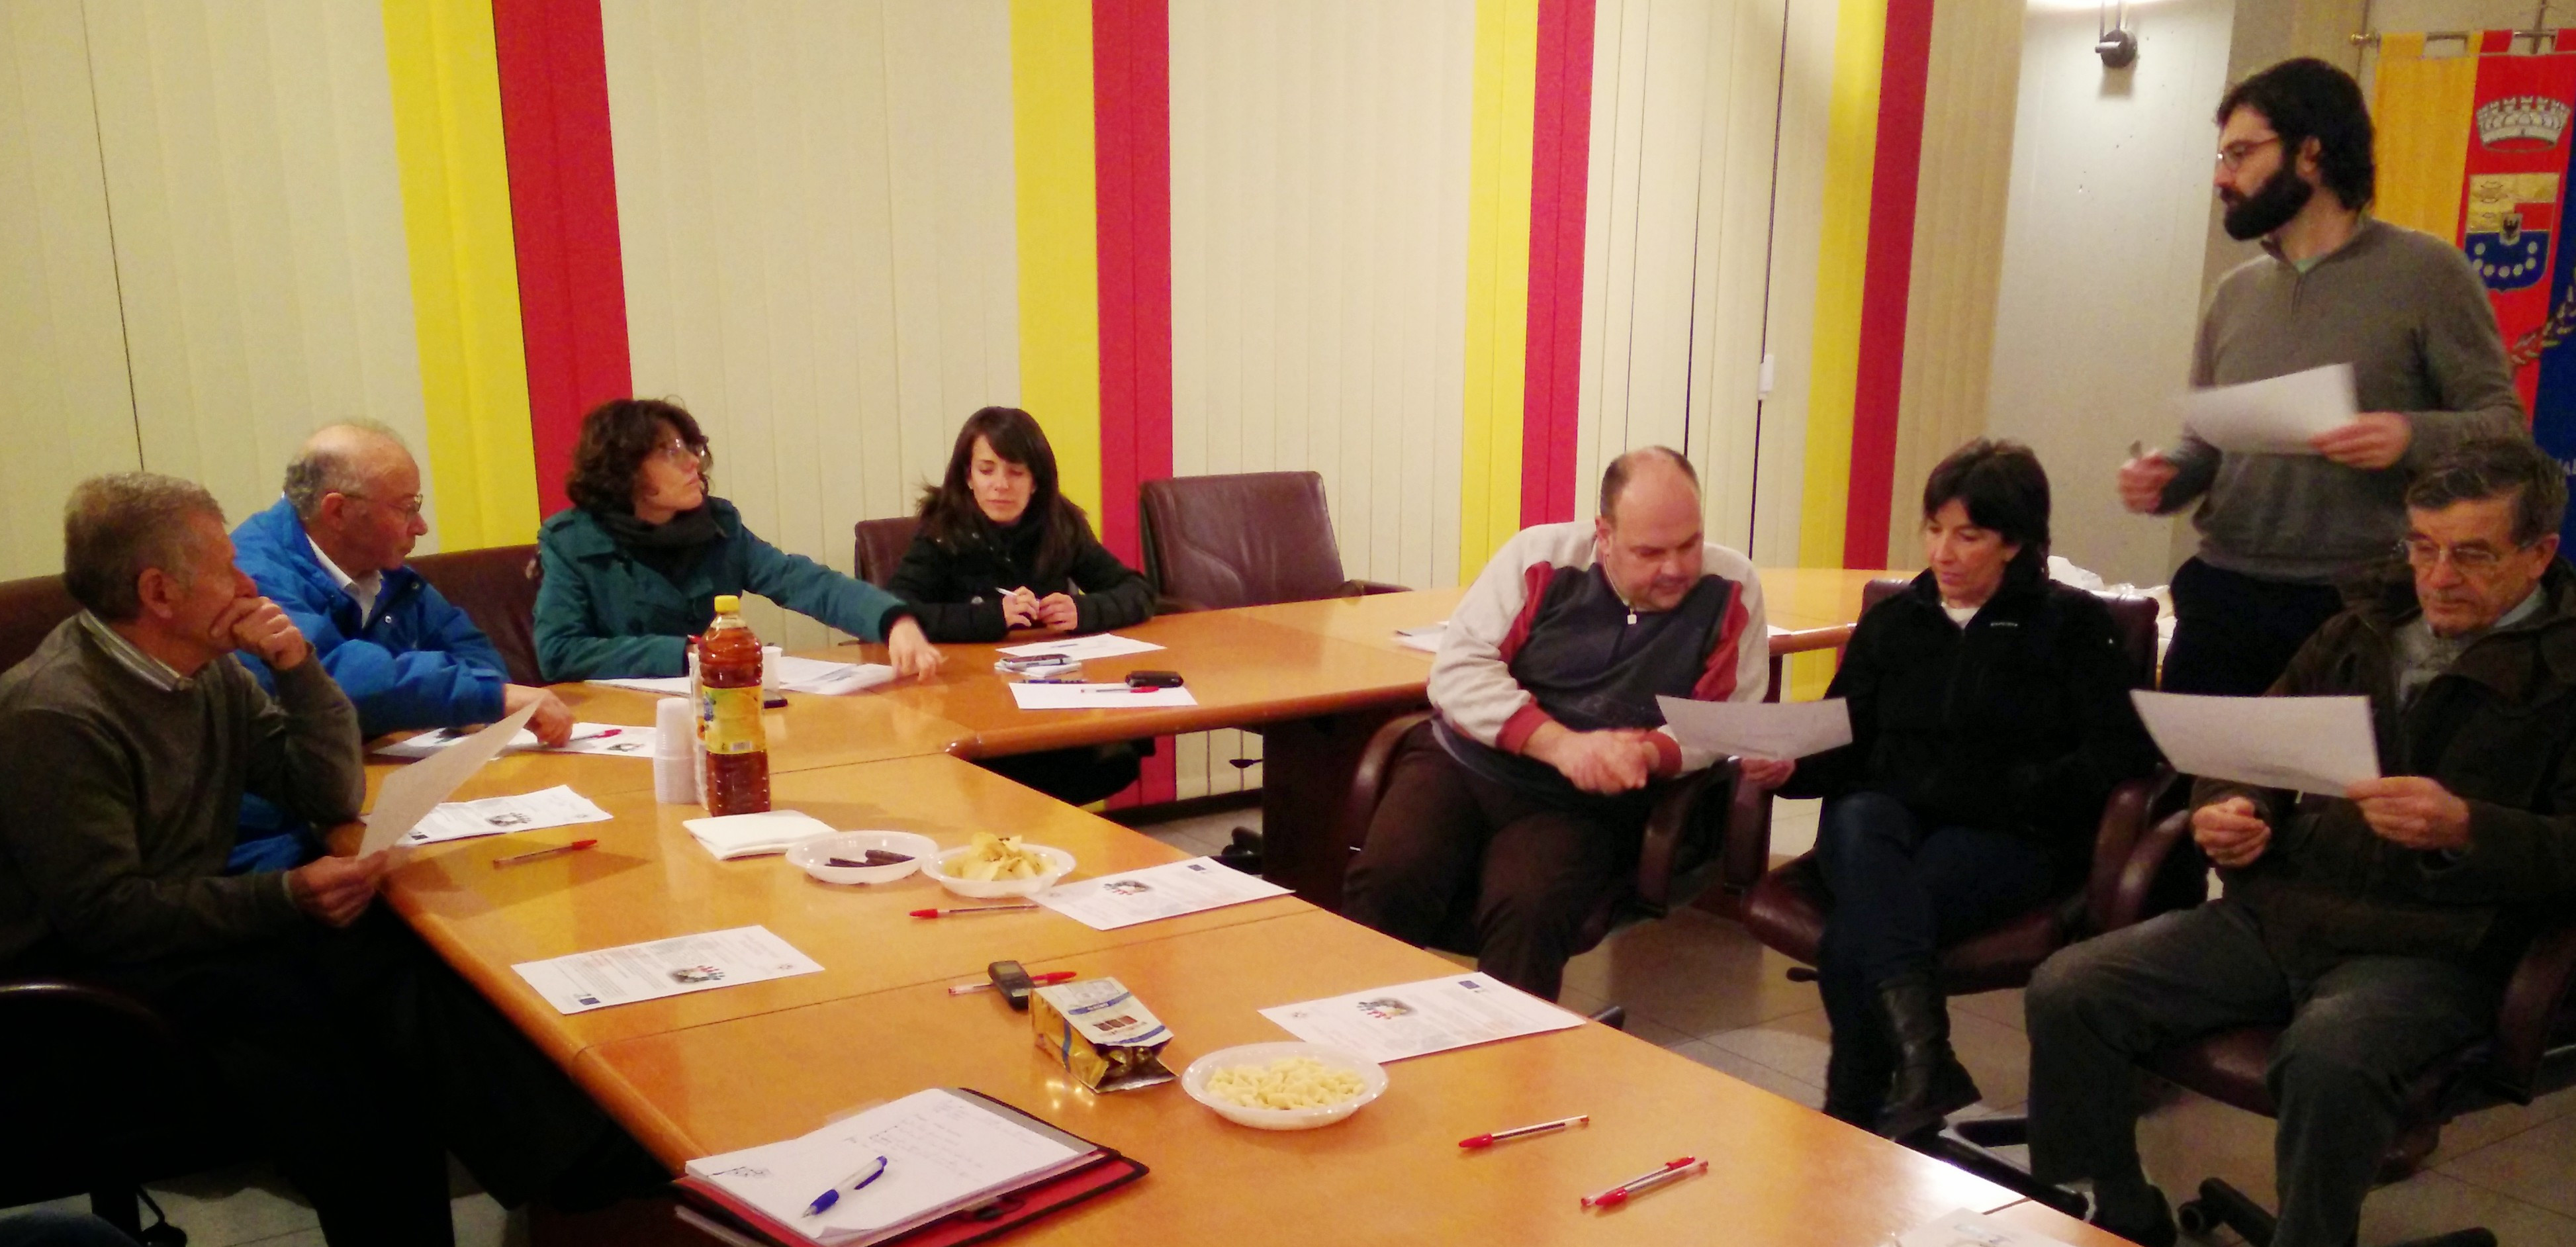
\includegraphics[width=.8\linewidth]{img/FocusGroup_TN.jpg}
	\caption{An initial moment of an exploratory focus group in Italy.}
	\label{fig:focusgroups}
\end{figure}


These activities involved potential and actual participant household members, recruited for the project, and they
were run as collective discussions. Usually they lasted around 2 hours and included between 6 and 8 discussants.
In case of the exploratory meetings, the scope of the discussion was intentionally broad and it aimed at revealing possible latent
needs or expectations, as well as discussing explicit ones. More importantly these were used to get first-hand knowledge
about the social and cultural environment where the platform was to be deployed. On the contrary, the evaluation discussions
had more specific focuses and involved concrete artifacts (\textit{e.g.} an interface mock-up or app prototype)
as a basis.

For instance, exploratory meetings helped us in putting in due perspective some of the features we initially taught
would be welcomed by end-users, such as `sharing' of energy performances or measurements typical of social network platforms.
In our contexts, it was both difficult to gfrasp the meaning of such a feature, bt it also raised
some concerns related to privacy. At the same time, the intermediate evaluation activities allowed us to spot some
limitations of our data visualizations (\textit{e.g.} oversimplifications of energy data through some charts),
and of the engagement and participatory process itself\footnote{A study of the end-users appreciation of the engagement and participatory process in the Italian pilots
is published in \cite{capaccioli_exploring_2017}.}
(\textit{e.g.} expectation of more frequent interactions with the project).


\subsubsection{Design workshops} % MAYBE TURN THESE INTO \PARAGRAPHS ?

\begin{figure}
      \begin{center}
        \begin{minipage}[htb]{0.43\linewidth}    
        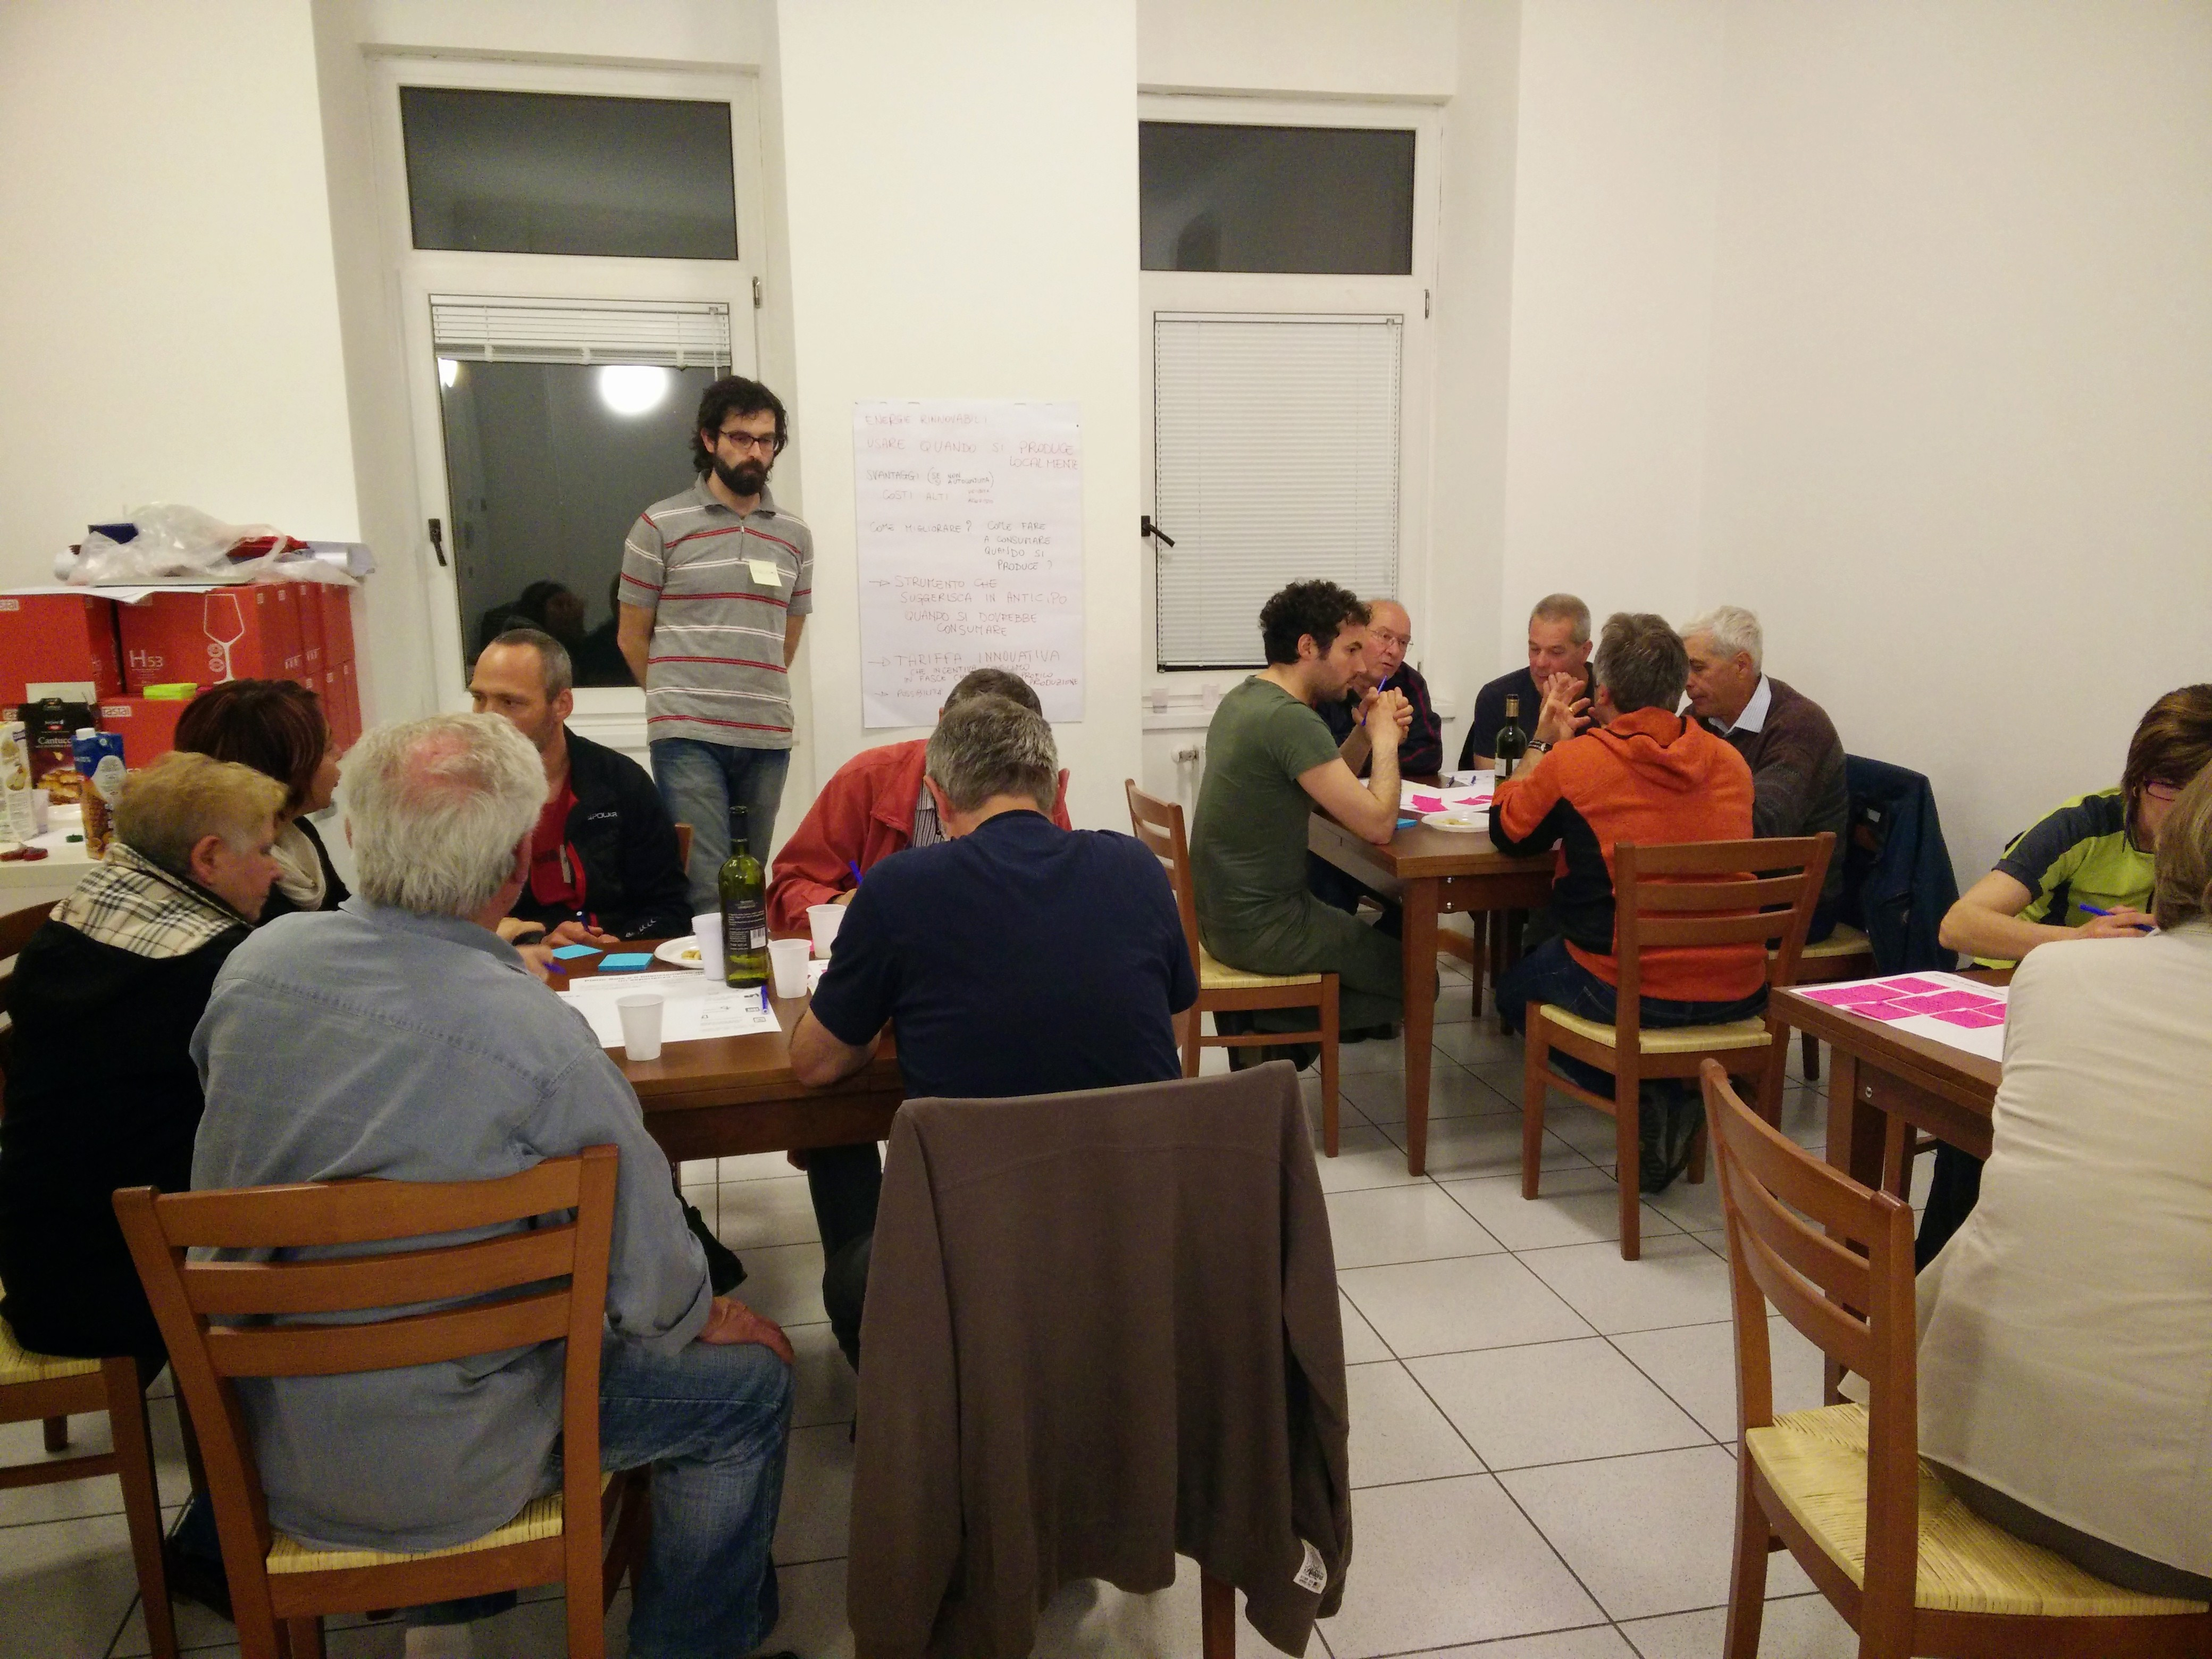
\includegraphics[width=1\linewidth]{img/Workshop_userreq1.jpg}
        \end{minipage}
 	\hfill 
         \begin{minipage}[htb]{0.55\linewidth}    
	        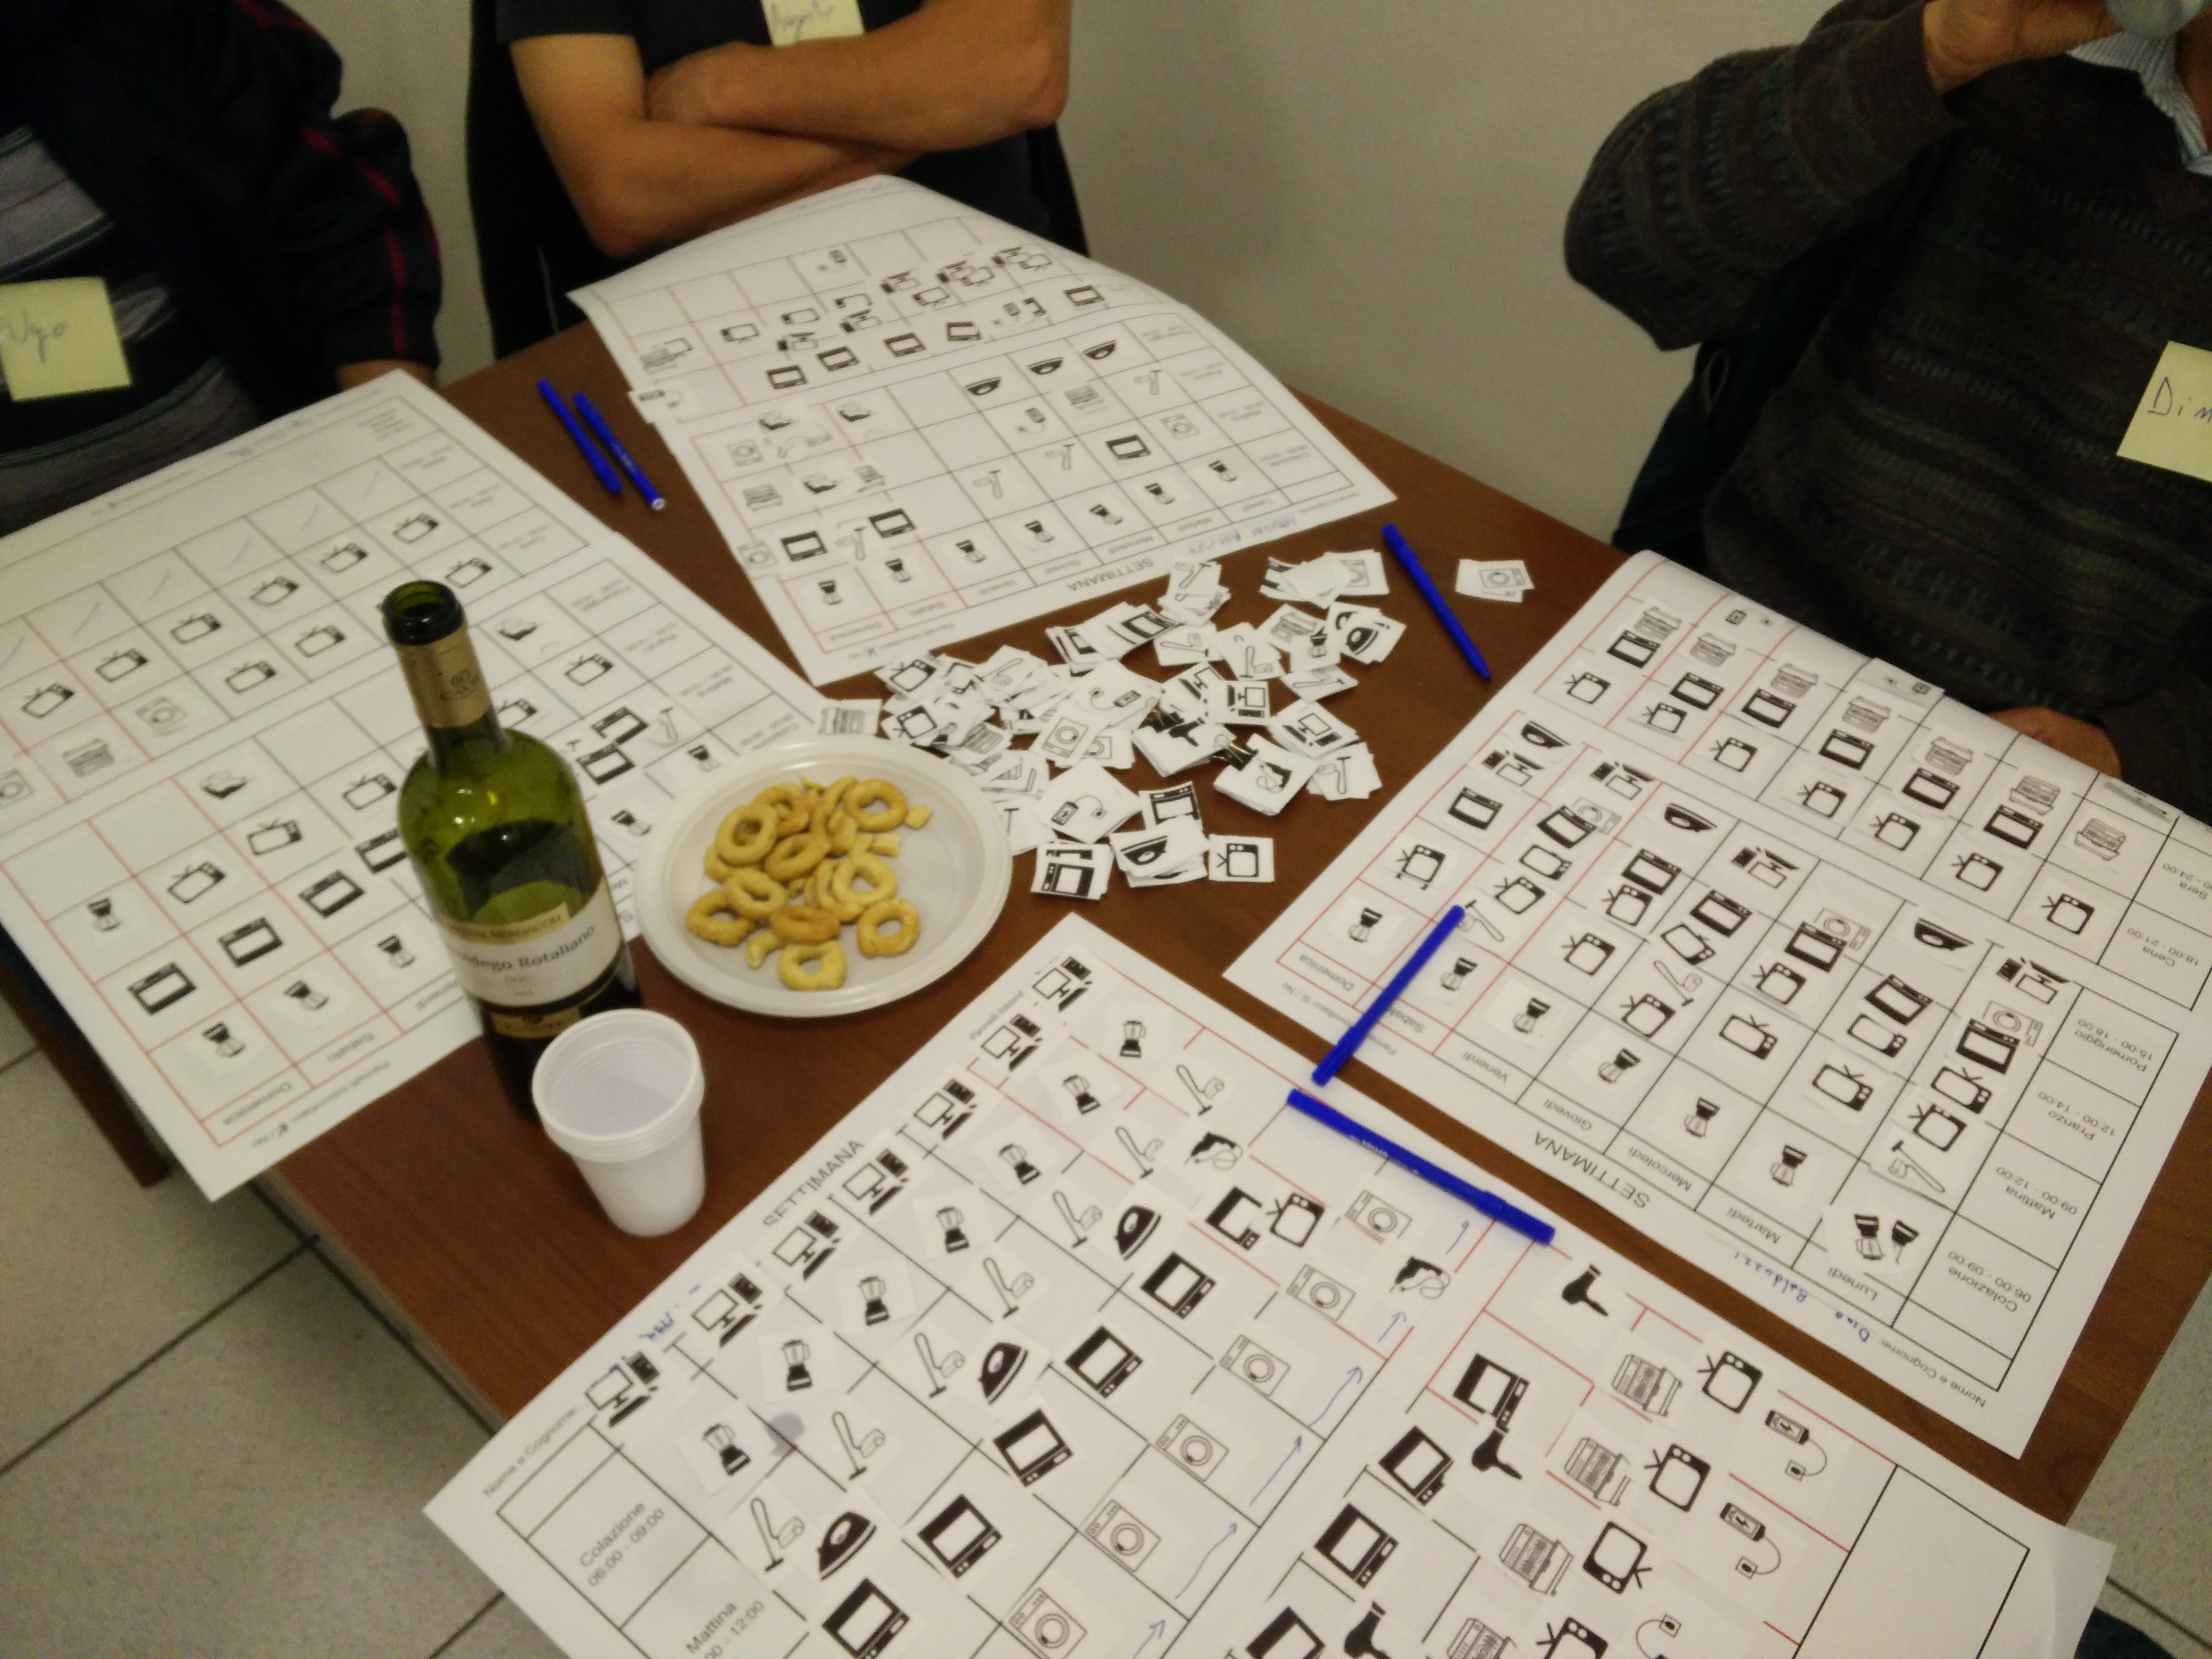
\includegraphics[width=1\linewidth]{img/Workshop_userreq2.jpg} 
                \end{minipage}
      \end{center}
    \caption{(a) Beginning of group activities in one of the first workshops held in Italy and focusing
    on user requirements; (b) One of the group outcomes for mapping energy consumption habits at home. 
}
\label{fig:workshops}
\end{figure}

These workshops involved concrete, hands-on activities done primarily with participant household members.
Occasionally a few workshops took place among project partners or had a broader target.
As it is typical of collaborative design approaches we adopted different workshop methodologies (\textit{e.g.} brainstorming, future scenarios,
collages, usage simulation) to suit diverse needs in the different phases of CIVIS.
Ultimately, they allowed to identify the end-user requirements\footnote{A preliminary analysis of these emerging requirements in the Italian pilots
is presented in \cite{capaccioli_participatory_2016}.} for the platform front-end as well as
improving and tailoring the interface layout.

For instance, for the module of \textit{Action suggestions}, the workshops were relevant for adjusting the various
tips for energy conservation to the local contexts of use. These were in fact quite different between the two countries,
 and certain tips had no meaning when delivered to one or another country or they needed a different
 rationale for their presentation.


\subsection{Main Outcomes of the Design Process} % Older heading ``Products of Design Process''
% \begin{svgraybox}
% [note by GP] Do we include here the main outputs only (I would suggest yes), or also the intermediate artifacts (mockups, user stories, etc...) of the process?
% \end{svgraybox}

\subsubsection{YouPower} %or similar heading
\begin{svgraybox}
\textbf{[IMPORTANT]} THIS IS JUST A PLACEHOLDER COPIED\&PASTED FROM CONF PAPER. \textit{IT NEEDS ADJUSTMENT}
\end{svgraybox}

\noindent Given time and resource constraints, the YouPower app can not be developed all-in-one cross-platform (for phones, tablets and computers). We chose to design the front-end as a hybrid mobile phone app, i.e. its UI design has layouts that suit phone screens, %The consideration is multi-fold. 
%Western Europe has a large mobile phone internet user base\footnote{Between 2013 and 2017, the penetration rate of mobile phone internet users among mobile phone users will rise from 49.0\% to 77.8\%. See more at: \url{ http://www.emarketer.com/Article/Nearly-Half-of-Western-Europeans-Will-Use-Mobile-Web-This-Year/1010510\#sthash.AaVfsqIU.dpuf}}. Many surveys show that mobile apps have advantages such as creating deeper user engagement, easy sharing, among others\footnote{\url{https://infomedia.com/blog/the-advantages-of-mobile-apps/}, \url{https://econsultancy.com/blog/62326-85-of-consumers-favour-apps-over-mobile-websites/}}. This makes mobile app a good choice given the goal of the CIVIS platform. 
since mobile apps can be more easily transformed to web browser versions, while the reverse is more difficult.
The back-end of the YouPower platform will remain mostly the same independent of the front-end alternatives.

CIVIS platform is composed of (I) the \textit{energy sensor level services} mainly
dealing with energy data collection; and (II) the \textit{energy data level and social
level services} mainly dealing with energy data analytics as well as user, household and community management
among others. 

\begin{figure}[h!]
\begin{center}\footnotesize
	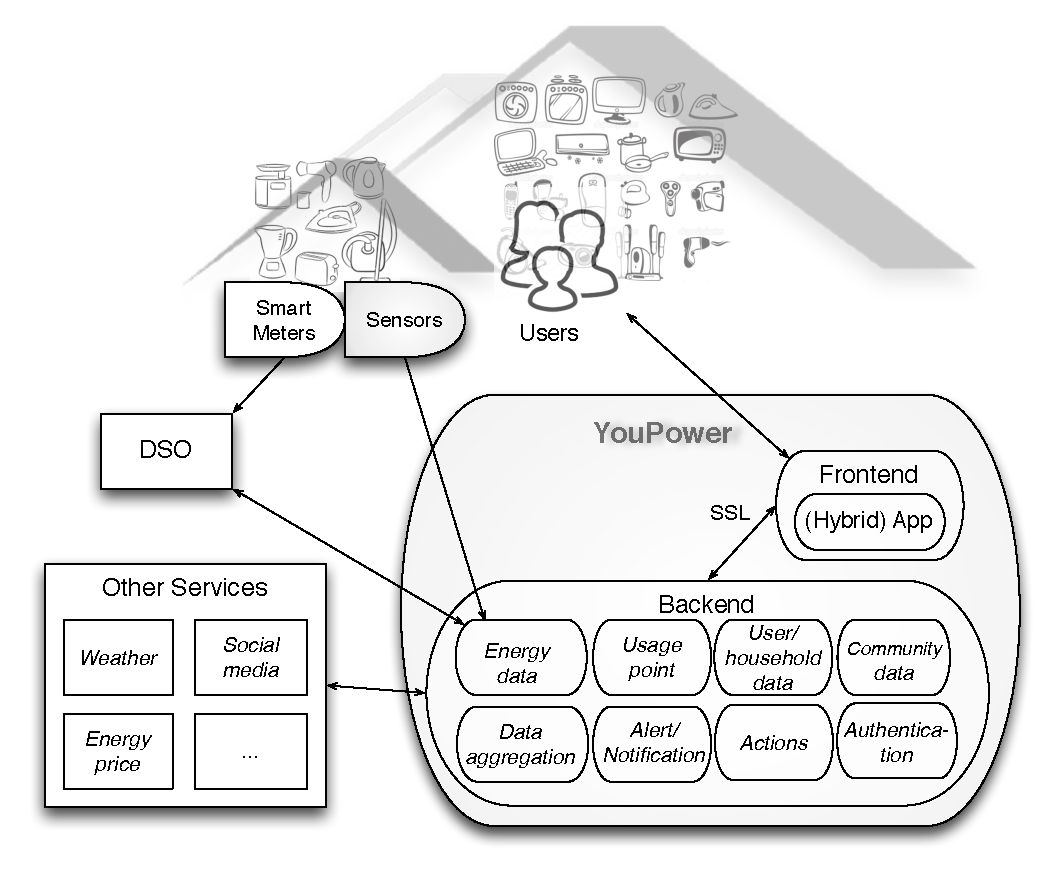
\includegraphics[width=1.0\linewidth]{img/civis_platform_overview.pdf}\\
	DSO (Distribution System Operators),  SSL (Secure Sockets Layer)
	\caption{YouPower Platform Overview}\label{fig:platform}
\end{center}
\end{figure}

(I) \textit{Energy sensor level services:} CIVIS project installed hardware (smart plugs and sensors) and
software required for appliance-level energy data collection. The hardware/software choices differ in the
two sites due to local circumstances. For example, \textit{Smappee}\footnote{\url{http://www.smappee.com}}
for 40 households in Stockholm, and \textit{CurrentCost}\footnote{\url{http://currentcost.com}} for 79
households in Trento. Trento also installed Amperometric clamps for PV prodcution measures. 
Household-level energy data is measured by smart meters and provided by local DSOs (Distribution System Operators). 

(II) \textit{Energy data level and social level services:} These services are provided by the YouPower
app and its back-end. The design of the YouPower app (and its back-end) consists of three self-contained
composable parts: (A) \textit{House Cooperatives} (contextualized and deployed to the Stockholm test site);
(B) \textit{Demand-Side Management} (contextualized and deployed
to the Trento test site); and (C) \textit{Action Suggestions} (contextualized and deployed to both test sites).


\paragraph{Housing Cooperatives}
% \label{sect:brf}

This part of the YouPower app is designed for the community of housing cooperatives (\textit{Bostadsr{\"a}ttsf{\"o}rening} or \textit{Brf} in Swedish) in the Stockholm test site \cite{Hasselqvist2016}.
Similar housing ownership and management models exist in a number of EU and non-EU countries, which allow potential wider application of the design.
A housing cooperative annually elects a board which manages cooperative properties and decides on energy contracts, maintains energy systems, and proposes investments in energy efficient technologies. Since board members are volunteers who may have limited knowledge of energy or building management, this part of the app aims to support board members in energy management, in particular energy reduction actions. Cooperative members can also use the app to follow energy decisions and works of the cooperative. Additionally, the app can be of interest by building management companies working with housing cooperatives. 
The information presented in the app is visible for these user
groups and shared between housing cooperatives. This openness of energy data is key to
facilitating  users in sharing experiences relevant for taking energy reduction actions.\\

% \subsubsection{Linking energy data to energy reduction actions}
\textbf{Linking energy data to energy reduction actions}

The design links energy data with energy reduction actions taken (Figure~\ref{fig:Figure201_Actions}), both at cooperative levels, making the impact of energy actions visible to users. The energy use is divided into heating \& hot water (from district heating), and facilities electricity (in apartment buildings). Users can switch between the views per month or per year to show overall changes. %Since the energy data is shared between cooperatives there may also be privacy concerns related to opening up data of higher granularity to people outside of the own cooperative. 
%
\begin{figure}[h!]
	\centering
	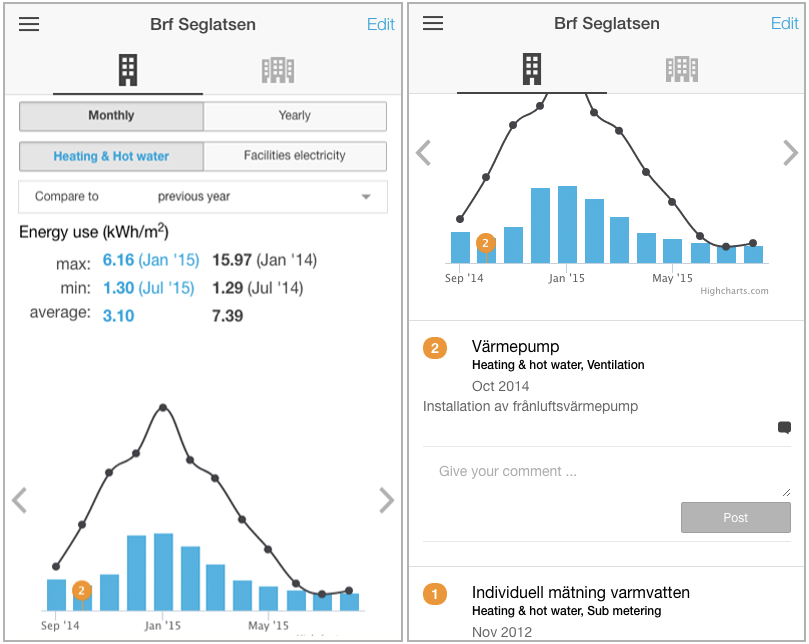
\includegraphics[width=.9\linewidth]{img/Figure201_Actions.png}
	\caption{Heasting \& hot water use graph. Blue bars show the current year's use per month; the black line shows that of previous year. Energy reduction actions taken are mapped to the time of action and listed below.}
	\label{fig:Figure201_Actions}
\end{figure}
%
Users with editing rights, typically board members, can  add energy reduction actions that the cooperative has taken, e.g., improvement of ventilation, lighting or heating systems, 
and the related cost.
Trusted energy or building management companies can also get editing rights to add energy reduction actions they took on behalf of the cooperative. 
Added actions appear at the month when each action was taken and are listed below the graph. When clicking on an action in the list, the details of the action are shown.
% 
To make the impact of actions visible, users can compare the energy use of the viewed months to that of a previous year. This can be used e.g. by a cooperative to explore what energy reduction actions to take in the future by learning actions taken by other cooperatives and what the effects were in relation to costs.\\

% \subsubsection{Comparing housing cooperatives}
\textbf{Comparing housing cooperatives}

\begin{figure}
	\centering
	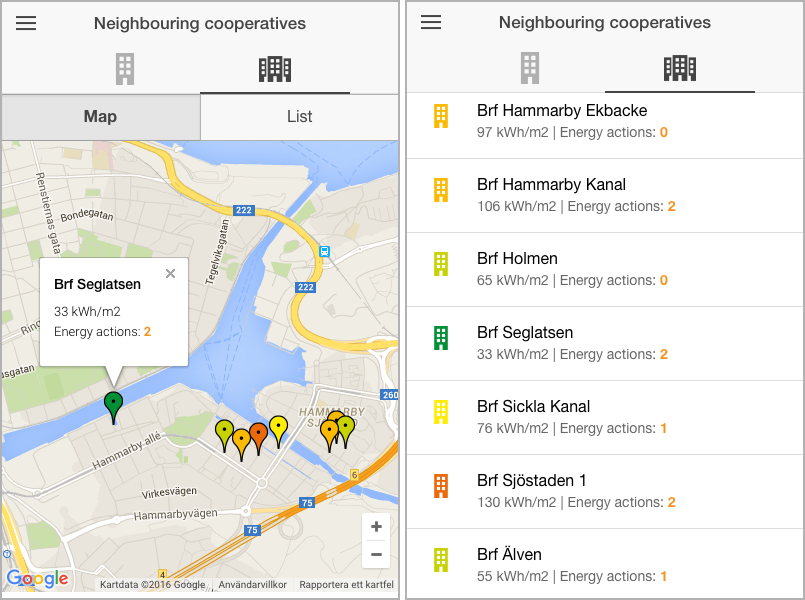
\includegraphics[width=0.9\linewidth]{img/Figure202_Housing_cooperatives_comparison.png}
	\caption{Map and list view of participating housing cooperatives. The energy performance of cooperatives is indicated by colour and in numbers.}
	\label{fig:Figure202_Housing_cooperatives_comparison}
\end{figure}

The cooperatives that are registered for the app are displayed in a map or list view (Figure~\ref{fig:Figure202_Housing_cooperatives_comparison}). Their icons are color coded (from red to green) based on each cooperative's energy performance, i.e. from high to low energy use per heated area, scaled according to the Swedish energy declaration for buildings\footnote{\url{http://www.boverket.se/sv/byggande/energideklaration/energideklarationens-innehall-och-sammanfattning/sammanfattningen-med-energiklasser/energiklasser-fran-ag/}}. 
%  but it is calibrated to only include measured energy use for heating and hot water, which is the greatest part of the energy use. In the Swedish energy declarations, facilities electricity is also added but that often requires estimations of different factors to make the number comparable.
% 
Users can also see the energy performance as a number (in kWh/m$^2$), and the information about energy reduction actions of the cooperatives. %The number of actions is important to display to make energy reduction efforts of housing cooperatives with a high energy performance (e.g. due to poor construction of the building) visible. 
% 
During stakeholder studies, energy managers in cooperative boards stressed the importance of knowing the difference between cooperatives in order to understand the difference in their energy performance. Thus, the design also includes information about cooperatives (Figure~\ref{fig:Figure204_Neighbourhood_average}) such as the number of apartments and heated areas in a cooperative, a building's construction year, and types of ventilations (e.g. with or without heat recovery).
% 
Users can compare a cooperative's energy use per month or per year to another cooperative or to the neighborhood average. The electricity use is also displayed per area (kWh/m$^2$) to make it comparable.\\
\begin{figure}
\centering
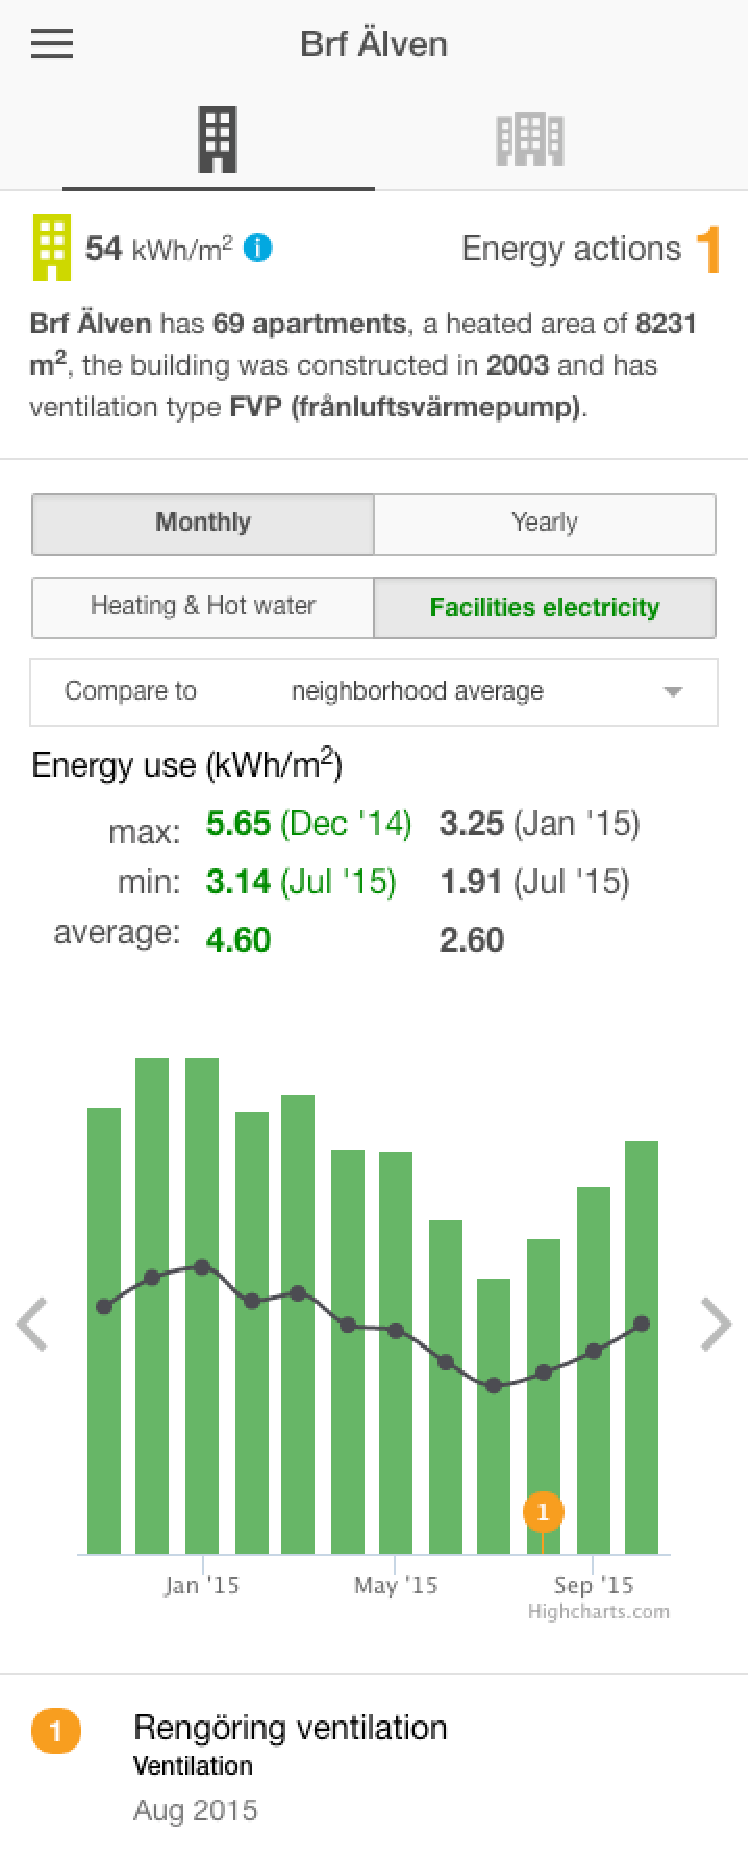
\includegraphics[width=.42\linewidth]{img/brf.pdf}
\caption{Facilities electricity use graph. Information about housing cooperatives and actions is displayed at the top. Green bars show the housing cooperative's current year's use per month; the black line shows the average use of all housing cooperatives}
\label{fig:Figure204_Neighbourhood_average} 
\end{figure}

% \subsubsection{Sharing experiences}
\textbf{Sharing experiences}


A cooperative interested in taking an action may wish to know more, e.g. which contractor was chosen for an investment and why or how to get buy-in from cooperative members. The design provides commenting functions for each action added, where users can post questions and exchange experiences. The cooperatives can also add email addresses of their contact persons, which are visible on each cooperative's app page.
% 
Sharing experiences certainly also happens outside of the digital world, e.g. during meetings of cooperative boards or with local energy networks. The app aims  to support discussions and knowledge exchange also in such situations, where someone can easily demonstrate the impact of an energy investment with smart phones.


% % % ITALIAN TEST SITE
\paragraph{Demand-Side Management} 
% \label{sect:load_shifting}

This part of the YouPower app is designed for the Trento test site and can have wider application.
It provides users historical and quasi real-time consumption and production information, and facilitates users to leverage load elasticity in order to maximize self-consumption of rooftop PV productions. 
Energy data is displayed at appliances (if smart plugs are installed), household, and electricity consortia levels. %to inform users of their own energy consumption patterns and those in the neighborhood. 
%
Consumption at the appliance level enables users to gain deeper understanding of their daily actions and the resulting energy use. 
% 
Historical and current consumption and production at the household level allow users to compare those two and potentially maximize self-consumption. 
% 
Aggregated and average consumption at the consortia level informs users of neighborhood energy consumption and allows comparisons.  
% 
In addition, dynamic Time-of-Use (ToU) signals are displayed  to assist users in load shifting during their daily actions. \\

% \subsubsection{Historical and quasi real-time consumption and production} 
\textbf{Historical and quasi real-time consumption and production}

At the household level, electricity consumption and PV production levels (in W and Wh) are displayed in quasi real-time and updated for the latest six minutes\footnote{For technical reasons such as households' data transfer connections and processing time, there can be up to 2-min delay between the time of actual power measurement and the data displayed.}.
This information can also be displayed as a bar chart for a chosen period (in the past) to provide an aggregated daily overview of consumption vs. production (Figure~\ref{fig:viz_rt}). 
% 
\begin{figure}
      \begin{center}
        \begin{minipage}[htb]{0.43\linewidth}    
        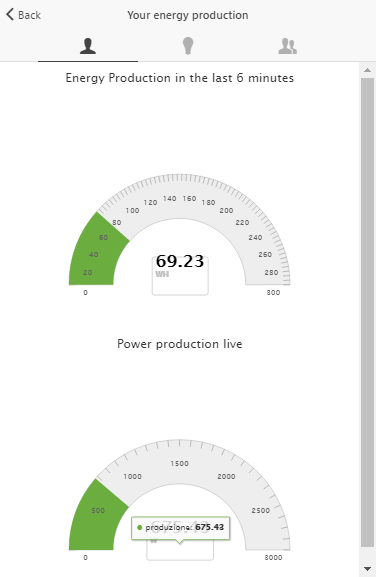
\includegraphics[width=1\linewidth]{img/visual_production.png}
        \end{minipage}
 	\hfill 
         \begin{minipage}[htb]{0.55\linewidth}    
	        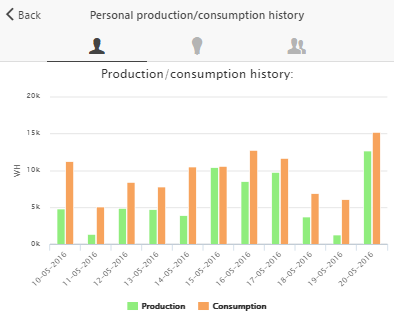
\includegraphics[width=1\linewidth]{img/historicalcomparison_prodcons.png} 
                \end{minipage}
      \end{center}
    \caption{(a) Quasi real-time meters for household PV production; (b) Household consumption vs. production for a chosen period
}
\label{fig:viz_rt}
\end{figure}
%
When smart plugs are installed, users can view the daily electricity consumption (in Wh) of the corresponding connected appliances of their own household for a chosen period (Figure~\ref{fig:viz_hist} a). This helps them to gain better insights into the individual appliance's consumption level and its daily or seasonal patterns. 
% Selection of data ranges are mandatory for these visualizations. They must be set by users at two different places: in the ``Energy Data'' main screen for the \textit{Household} category; in the ``light-bulb'' sub-view for the \textit{Appliance} one, which is accessible from the top level bar.
\begin{figure}
      \begin{center}
        \begin{minipage}[htb]{0.54\linewidth}    
        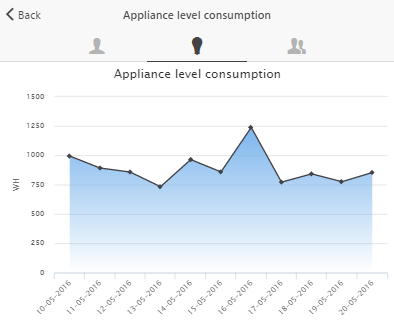
\includegraphics[width=1\linewidth]{img/applianceconsumption.png}
        \end{minipage}
	\hfill 
        \begin{minipage}[htb]{0.44\linewidth}    
         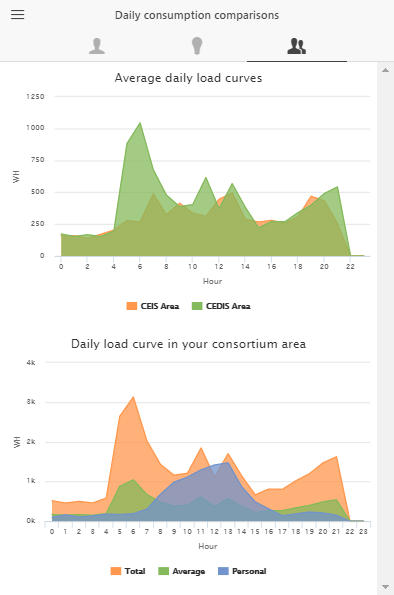
\includegraphics[width=1\linewidth]{img/benchmark.png}
        \end{minipage}
      \end{center}
      \caption{(a) Daily electricity consumption at the appliance level for a chosen period;  (b) 
      A household's hourly consumption profile over a chosen day compared to the averages and totals of the consortia
}
\label{fig:viz_hist}
\end{figure}
 %
With the aggregated energy data provided by the two local electricity consortia, users can also  compare their own households' hourly consumption profiles over a chosen day to the averages and totals of the consortia to gain a sense of their relative performance compared to their peers (Figure~\ref{fig:viz_hist} b). \\

\begin{figure}
      \begin{center}
        \begin{minipage}[htb]{0.45\linewidth}    
        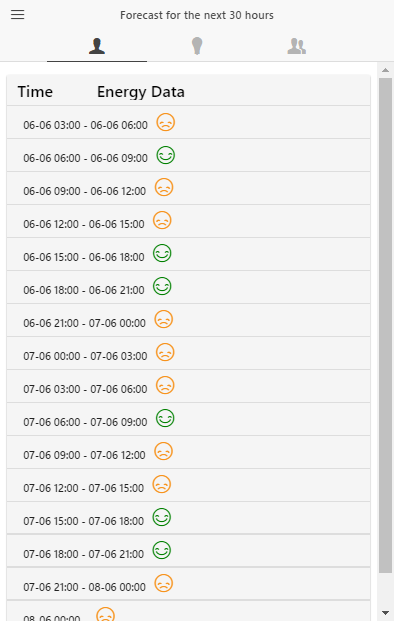
\includegraphics[width=1\linewidth]{img/touprediction.png}
        \end{minipage}
	\hfill 
        \begin{minipage}[htb]{0.45\linewidth}    
         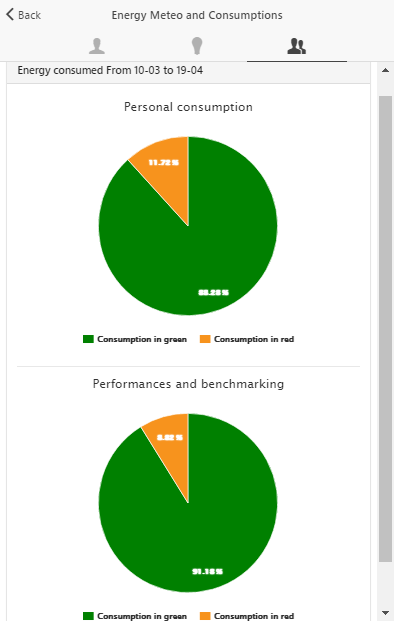
\includegraphics[width=1\linewidth]{img/touperformancechart_indivcoll.png}
        \end{minipage}
      \end{center}
      \caption{(a) Dynacmie ToU signals at 3-hour intervals for the forthcoming 30 hours;  (b) 
      A household's hourly consumption profile over a chosen day compared to the averages and totals of the consortia
}
\label{fig:tou}
\end{figure}

% \subsubsection{Dynamic ToU signals} 
\textbf{Dynamic ToU signals}

Dynamic ToU signals are provided to facilitate users' self-consumption of local PV productions.
They give clear indications to encourage or discourage electricity consumption at a certain moment based on the forecasted local renewable production level calculated with open weather forecast information (in particular solar radiation data) and the local rooftop PV production capacity. 
The signals are at 3-hour intervals for the forthcoming 30 hours (Figure \ref{fig:tou} a), and are updated every 24 hours. A green smiley face signals a time slot suitable for self-consumption where the forecasted local PV production exceeds the current local consumption, while an orange frown face signals otherwise.  
% 
On a weekly basis, users get a summary of the proportion of their own household consumption that took place under green or orange ToU signals to allow them to reflect on their levels of self-consumption (Figure \ref{fig:tou} b). The same information is also provided at the consortia level to enable peer comparison. 


\paragraph{Action Suggestions}
% \label{sect:tips}

This part of the YouPower app aims to %provide actionable suggestions to 
facilitate all household members to take part in energy conservation in their busy daily life. 
% 
About fifty action suggestions are composed to provide users practical and accurate information about energy conservation. 
They include one-time actions such as ``Use energy efficient cooktops'', routine actions such as ``Line dry, air dry clothes whenever you can'', as well as in-between actions (reminders) such as ``Defrost your fridge regularly (in $x$ days)''. 
Some suggestions may seem obvious and trivial, but as indicated by literature, people often has an attitude-behavior gap when it comes to environmental issues. The goal is to facilitate the behavior change process to bridge the attitude-behavior gap, making energy conservation new habits integrated in everyday household practices. 

% \subsubsection{Free choice and self-monitoring of energy conservation actions}
\textbf{Free choice and self-monitoring of energy conservation actions}

The actions are not meant as prescriptions for what users should do but to present different ideas of what they can do (and how) in household practices. 
Users can freely choose whether (and when) to take an action and possibly reschedule and repeat the action according to the needs and interests in their own context (Figure \ref{fig:actions}). After all, users are experts of their own reality. They also have an overview of their current, pending, and completed actions.
A new action is suggested when one is completed. %After an action is in progress, the user may also postpone, abandon or indicate that the action is completed (Figure \ref{fig:actions} c). 
When an action is scheduled, its reminder is triggered by time. Users' own choices of actions and the action processes facilitate the sense of autonomy which enhances and maintains motivation \cite{Ryan2000}. \\

\begin{figure}[b!]
      \begin{center}
        \begin{minipage}[t!]{0.33\linewidth}
	       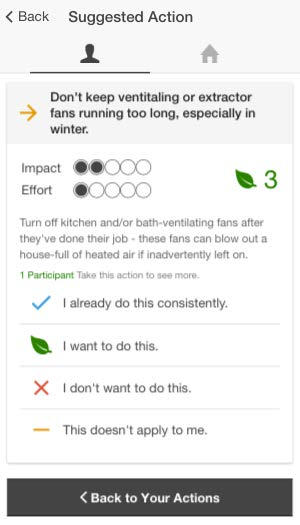
\includegraphics[width=1\linewidth]{img/action_details.jpg}
        \end{minipage}
        \begin{minipage}[t!]{0.31\linewidth}
        	       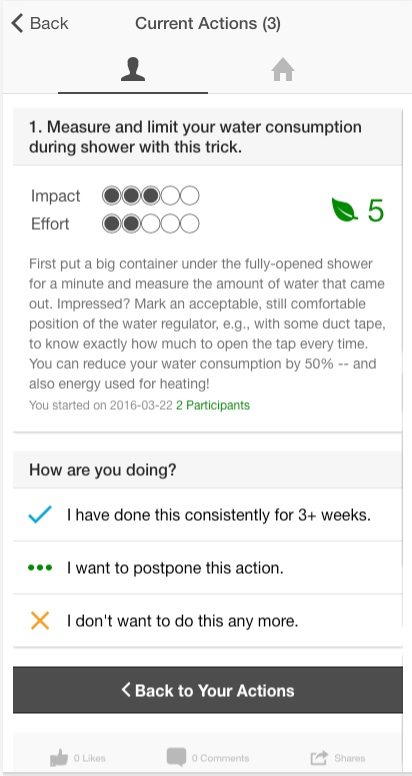
\includegraphics[width=1\linewidth]{img/Your_Actions.jpg}
                \end{minipage}
        %\hfill 
        \begin{minipage}[t!]{0.33\linewidth}    
         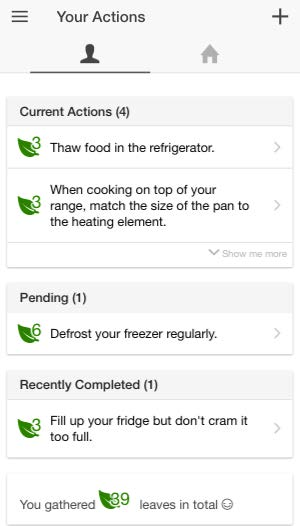
\includegraphics[width=1\linewidth]{img/action_tab.jpg}    
        \end{minipage}
      \end{center}
      \caption{(a) Action suggestion; (b) Action in progress; (c) User actions}\label{fig:actions}
\end{figure}


% \subsubsection{Promoting motivation and engagement} 
\textbf{Promoting motivation and engagement}

The design uses a number of elements to promote users' motivation and engagement. 
The suggestions are tailored to the local context by local partners and focus groups. 
Each action is accompanied by a short explanation, the entailed effort and impact (on a five-point scale) and the number of users taking this action. 
The design encourages users to take small steps (and not to have too many actions at a time) and gives positive performance feedback. 
In addition, users can invite household members, %  (Figure \ref{fig:invite}), 
view and join the energy conservation actions of the whole household (Figure \ref{fig:form} a).
Users can also login with Facebook, like, comment, share actions, % (Figure \ref{fig:share}), 
give feedback (Figure \ref{fig:form} b c) and invite friends. Users are awarded with points  (displayed as Green Leaves) once they complete an action, or provide feedback or comments. 


\begin{figure}
      \begin{center}
      \begin{minipage}[t!]{0.33\linewidth}    
               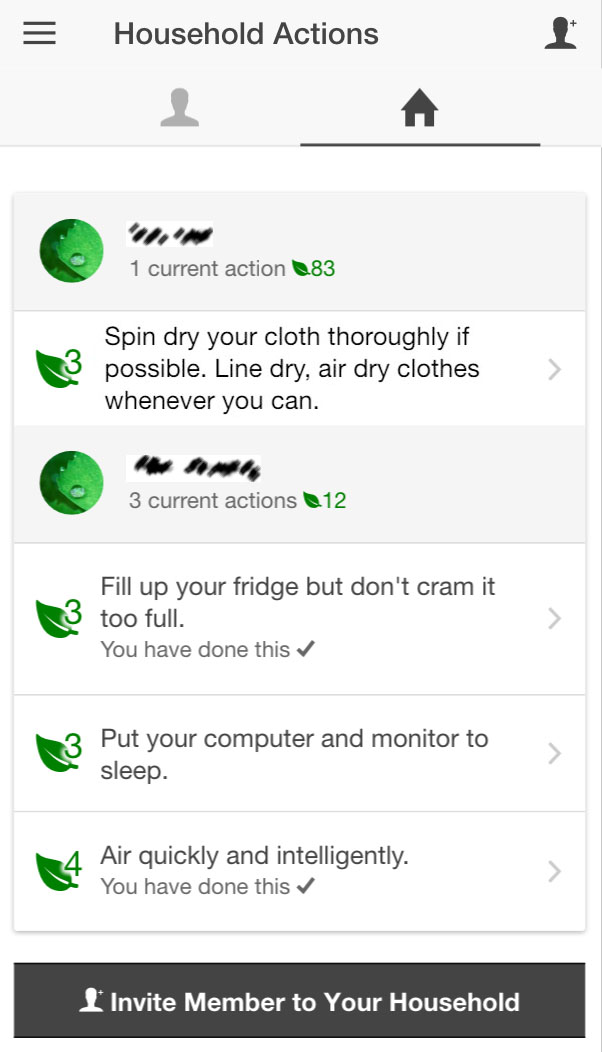
\includegraphics[width=1\linewidth]{img/house2.jpg}    
       \end{minipage}
        \begin{minipage}[t!]{0.33\linewidth}
	       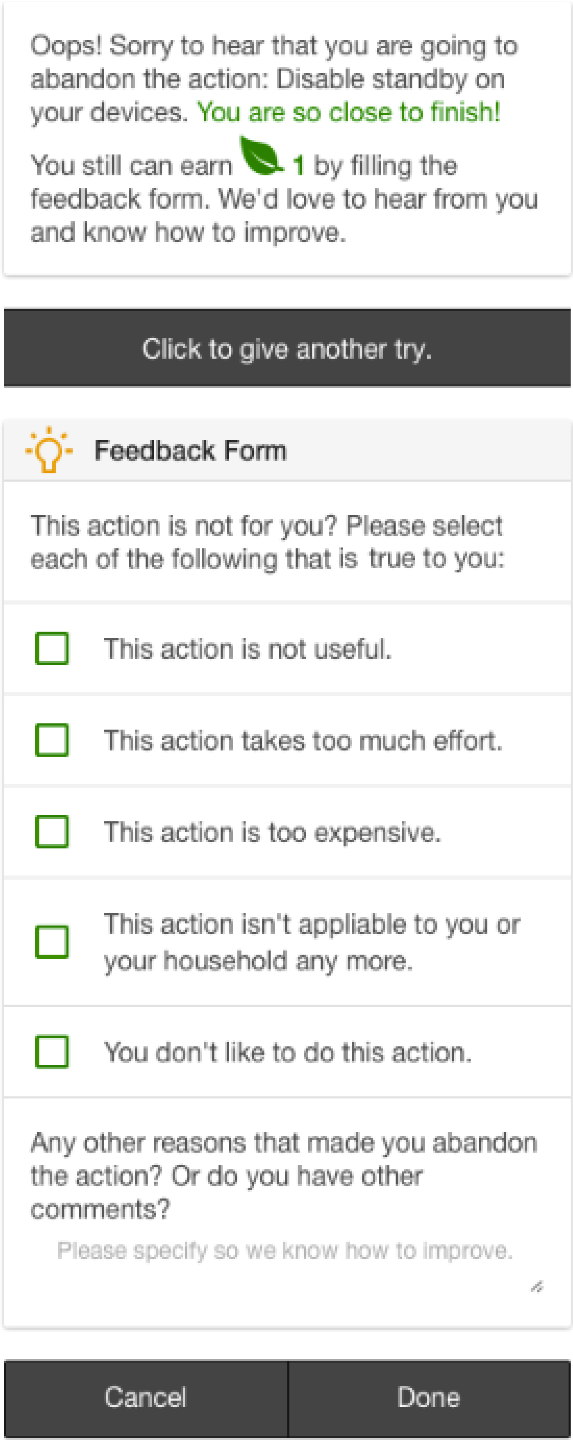
\includegraphics[width=1\linewidth]{img/action_not_completed.pdf}
        \end{minipage}
        \begin{minipage}[t!]{0.31\linewidth}
        	       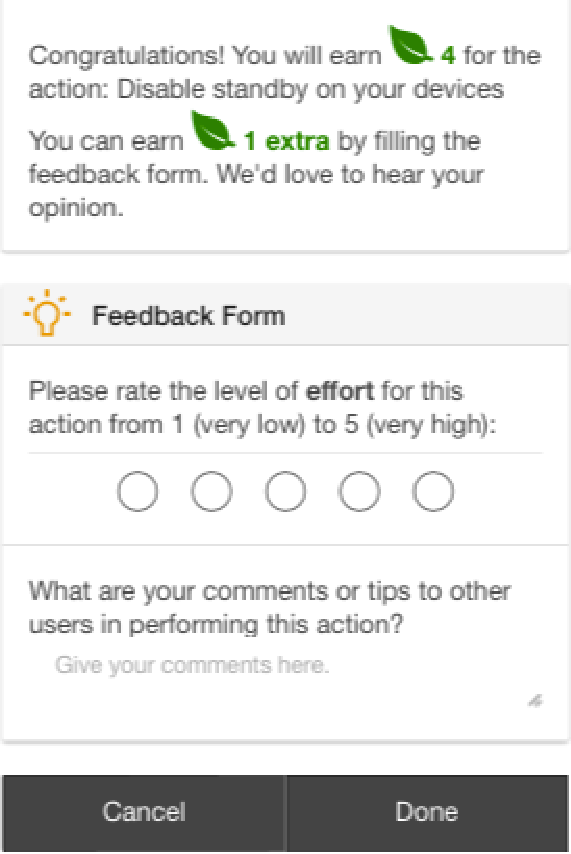
\includegraphics[width=1\linewidth]{img/action_completed.pdf}
                \end{minipage}
        %\hfill 
      \end{center}
      \caption{(a) Household actions; (b) Feedback form -- action abandoned; (c) Feedback form -- action completed}\label{fig:form}
\end{figure}



\subsubsection{Community Engagement Approaches (or models)} %or another nicer subsec-heading
% \begin{svgraybox}
% [note by GP] Participatory energy budgeting process in trento + Training sessions 
% in sweden (if you find any info about these Swe activities - from deliverables or kth publications, 
% please send me a note).
% \end{svgraybox}

Another main outcome of the design process, which also reflects the potential richness of designing for large scale
socio technical systems, rests at the level of community engagement. Indeed, approaches to the
use, adoption and appropriation of the platform resulted for the pilots in the two countries. Indeed, 
the ambition to foster energy behavioural changes at the collective level of communities (or neighborhoods),
instead of simply aiming for individual technology adoption, it made clear the need to design for
this too.

In the two national contexts, two different engagement processes which tried to stimulate the
emergence of the social dynamics connected to change of energy behaviour accompanied the technology deployment
and testing. 

In Italy, a full fledged process named \textit{participatory energy budgeting} (PEB) \cite{capaccioli_exploring_2017,capaccioli_exploring_2016}
was run for the management and allocation of an energy bonus, collected through the collective effort
of shifting demand toward hours of production peaks. Similarly to the original participatory budgeting,
the process aims at promoting participation and decision making for the allocation of part of a public budget, however,
instead of using public funds, it used an `energy bonus' generated through community performances in load shifting. 
Youpower's module on Demand-side management would help participants to maximize such performance and therefore, increase the energy bonus
to be managed collectively at the end of the PEB experience.

% TEXT BY HANNA H
In Sweden, the engagement work and app design aimed to complement the already existing community efforts to address energy issues. Meetings were arranged with housing cooperative representatives to discuss experiences of energy reduction actions and how those could be shared through the Youpower app. Furthermore, the app was used as a probe to discuss housing cooperative energy management with other stakeholders who may influence housing cooperative energy use, such as building managers, energy providers, and energy advisors. These stakeholders were already working with housing cooperatives and many had ambitions of supporting housing cooperatives in reducing energy use. By engaging with these stakeholders and learning about their processes and goals, we identified opportunities for the Youpower app, or similar tools, to be used jointly by these stakeholders and housing cooperatives to support energy improvement work.

\section{Discussions} %Shouldn't this be a separated file?
\label{sec:disc}

\begin{svgraybox}
Lessons Learned?  / Design Guidelines? 
\end{svgraybox}


\section{Discussions}

Collaboratively designed with the stakeholders from different pilot sites, the main outcomes of CIVIS addressed the goals and context of the project at different ST levels. They include the CIVIS platform consisted of YouPower, an open source social smart grid application, and the corresponding hardware and software installation for energy data collection at participating households from the pilot sites. The   deployment was accompanied by community engagement approaches to ensure that the stakeholders were well aware of the key issues and results the project was aiming at, and to develop positive attitude and encourage active participation. 
% 

At the Italian pilot sites, self-consumption of local renewable production was promoted at household and consortium levels, while at the Swedish pilot sites, knowledge sharing about housing cooperatives energy management practices was supported among cooperatives' board members and across different cooperatives. To bridge the attitude-behaviour gap of people's environmental values (and attitudes) and their actual behaviour in energy consumption \cite{Kollmuss2002,Schultz2002,Schultz2014}, the platform also provided a set of features that could facilitate users' behaviour change process towards sustainable  consumption that was implementable in their daily life along their existing practices. 
% 
In the following, we discuss a number of lessons learned from the CIVIS design experience, which could also be relevant to the design of other smart urban ecosystems beyond the particular case of CIVIS project. 
% 

First, despite the many advantages already discussed previously, implementing a collaborative participatory design process is highly challenging in practice with an interdisciplinary team in an international setting. The design and development team, together with stakeholders involved, have various professional and cultural backgrounds, possibly speak diverse languages, hold disparate values and principles, work in different styles, not to mention the personal and organizational interests they may withhold. Misunderstandings on terminologies,  methodologies and actions may go unnoticed and accumulate until it is very challenging or even critical to mediate the diverging opinions. The full awareness of such issues, frequent and efficient communications,  positive and constructive attitude, plus open-mindedness are the keys to make the development process effective and enjoyable.
% 

Second, do not underestimate the relevance, importance and challenge of setting up an engagement strategy or change process for the potential users of the new or modified system.
Engaging people in changing behaviours has much to do with understanding local contexts, people's heterogeneous attitudes, and local cultures. It also needs careful planning and execution.
Develop a clear engagement strategy starting from the beginning of the project and let the professionals with the proper skills in this area to interact with the stakeholders. 
% 

Third, with respect to STS design and engagement strategies, provide users and other stakeholders accurate and actionable information about how to achieve the  target behaviour. At the CIVIS pilot sites, for example,  people expressed the desire and need to do more for a sustainable future. They like the idea of receiving relevant and contextual suggestions and tips for action. Given the heterogeneity of the potential stakeholder groups, understanding them and their interests and needs remains a crucial and challenging part of design that requires careful confrontation with stakeholders directly.
% 

Fourth, foster consumers' intrinsic motivation for engagement. Allow users to freely practice and adapt their courses of actions. This facilitates the sense of competence and autonomy which promotes and enhances motivation for behaviour change \cite{Ryan2000}. 
For example, people in the pilot sites are skeptical about how much monetary gains they can actually have by using less energy in households, but they are driven by intrinsic motives as well as altruistic and environmental values for energy saving. The social and community-oriented features as those designed in the CIVIS project  articulate those values. 

With the explosive growth of smart devices and smart everything, the coming wave of  IoT and the hyperconneted world will soon bring the society into a smart environment where computing is pervasive \cite{gubbi2013internet,Shin2014}. Will this smartness bring its inventors and the natural world into a sustainable future? This chapter wishes to advocate that the fruitfulness of IoT and smart urban ecosystems do not mainly rely on the technological side as is the case with other STS. Designers and engineers need to indispensably take a human-centred ST approach in developing a smart sustainable future.   


% is designed and developed as a set of open source packages that are composable and extensible (under Apache v.2 license) to different needs related to energy conservation and load shifting interventions. The development was completed by June 2016, and different parts were deployed to the test sites in Stockholm and Trento respectively. 
%The initial deployment of YouPower shows that household engagement varies significantly between test sites and among participants. The main reason for this can probably be found in the different characteristics of the communities: elderly people and parents with older children (mainly in the Italian test site) in particular participated enthusiastically, while a much smaller number of families with young children (mainly in the Swedish test site) participated actively in the project. Preliminary results seem to suggest that engagement can be driven not only by individuals' pre-existing motivations (e.g., financial or environmental) but also by households' experiences and interactions once they start actively using an application such as YouPower. We conjecture that more engagement of users will lead to more energy reductions. % and ultimately a more sustainable world. More research is needed to support this conclusion, which is left for future work. 
%While the initial deployment of YouPower shows that household engagement varies significantly between the two test sites and among participants, preliminary results do suggest that a community-oriented intervention, such as YouPower, increases user engagement significantly.
%, particularly for elderly people and parents with older children. 
%The results suggest that engagement can be driven not only by individuals' pre-existing motivations (e.g., financial or environmental) but also by households' experiences and interactions once they start actively using an application such as YouPower. We conjecture that more user engagement will lead to more energy reductions and better load-shifting results. % and ultimately a more sustainable world. 
% More research is needed to support this conclusion, which is left for future work.
%An extended data collection period for the households' energy consumption data at the test sites is needed (to obtain an annual energy consumption pattern during the intervention period to be compared to pre-intervention period data) for the research to draw a conclusion on the effect of the intervention on energy consumption behaviour in the test sites. This effort is left for future work.





\begin{figure}[b]
\sidecaption[b]
% Use the relevant command for your figure-insertion program
% to insert the figure file.
% For example, with the option graphics use
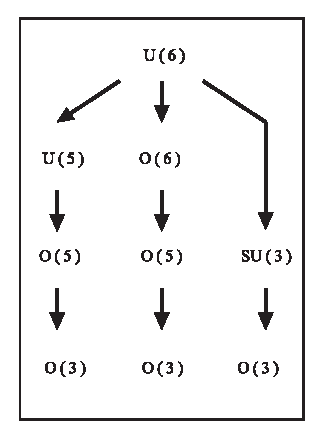
\includegraphics[scale=.65]{figure}
%
% If no graphics program available, insert a blank space i.e. use
%\picplace{5cm}{2cm} % Give the correct figure height and width in cm
%
%\caption{Please write your figure caption here}
\caption{If the width of the figure is less than 7.8 cm use the \texttt{sidecapion} command to flush the caption on the left side of the page. If the figure is positioned at the top of the page, align the sidecaption with the top of the figure -- to achieve this you simply need to use the optional argument \texttt{[t]} with the \texttt{sidecaption} command}
\label{fig:2}       % Give a unique label
\end{figure}


\subruninhead{Run-in Heading Italic Version} Use the \LaTeX\ automatism for all your cross-refer\-ences and citations as has already been described in Sect.~\ref{sec:2}\index{paragraph}.
% Use the \index{} command to code your index words
%
\begin{table}
\caption{Please write your table caption here}
\label{tab:1}       % Give a unique label
%
% Follow this input for your own table layout
%
\begin{tabular}{p{2cm}p{2.4cm}p{2cm}p{4.9cm}}
\hline\noalign{\smallskip}
Classes & Subclass & Length & Action Mechanism  \\
\noalign{\smallskip}\svhline\noalign{\smallskip}
Translation & mRNA$^a$  & 22 (19--25) & Translation repression, mRNA cleavage\\
Translation & mRNA cleavage & 21 & mRNA cleavage\\
Translation & mRNA  & 21--22 & mRNA cleavage\\
Translation & mRNA  & 24--26 & Histone and DNA Modification\\
\noalign{\smallskip}\hline\noalign{\smallskip}
\end{tabular}
$^a$ Table foot note (with superscript)
\end{table}

\begin{description}[Type 1]
\item[Type 1]{That addresses central themes pertainng to migration, health, and disease. Blablabla}
\item[Type 2]{That addresses central themes pertainng to migration, health, and disease. Blablabla}
\end{description}





\begin{acknowledgement}
If you want to include acknowledgments of assistance and the like at the end of an individual chapter please use the \verb|acknowledgement| environment -- it will automatically render Springer's preferred layout.
\end{acknowledgement}
%
%\section*{Appendix}
%\addcontentsline{toc}{section}{Appendix}
%


%%%%%%%%%%%%%%%%%%%%%%%% referenc.tex %%%%%%%%%%%%%%%%%%%%%%%%%%%%%%
% sample references
% %
% Use this file as a template for your own input.
%
%%%%%%%%%%%%%%%%%%%%%%%% Springer-Verlag %%%%%%%%%%%%%%%%%%%%%%%%%%
%
% BibTeX users please use
\bibliographystyle{abbrv}
\bibliography{bib,bib_gp}
%

%\begin{thebibliography}{99.}%
% and use \bibitem to create references.
%
% Use the following syntax and markup for your references if 
% the subject of your book is from the field 
% "Mathematics, Physics, Statistics, Computer Science"
%
% Contribution 
%\bibitem{science-contrib} Broy, M.: Software engineering --- from auxiliary to key technologies. In: Broy, M., Dener, E. (eds.) Software Pioneers, pp. 10-13. Springer, Heidelberg (2002)
%
% Online Document

%\end{thebibliography}

\end{document}
